%
% Modelo de trabalho acadêmico (Teses, Dissertações, TCC)
% Documento principal
%
% Centro Federal de Educação Tecnológica de Minas Gerais - CEFET-MG
% Autor: Cristiano Fraga G. Nunes <cfgnunes@gmail.com>
%
% Projeto hospedado em: https://github.com/cfgnunes/latex-cefet-mg
%
%
% Informações:
%   Codificação utilizada: UTF-8
%   Tamanho da tabulação: 4 (espaços)


\documentclass[oneside]{abntex2-cefetmg}            % Imprimir apenas frente
%\documentclass[doubleside]{abntex2-cefetmg}        % Imprimir frente e verso

% Importações de pacotes
\usepackage[portuguese, onelanguage, lined, boxed, commentsnumbered, algoruled]{algorithm2e}                % Escrever algoritmos
\usepackage[alf, abnt-emphasize=bf, bibjustif, recuo=0cm, abnt-etal-cite=2, abnt-etal-list=0]{abntex2cite}  % Citações padrão ABNT
\usepackage[utf8]{inputenc}                         % Acentuação direta
\usepackage[T1]{fontenc}                            % Codificação da fonte em 8 bits
\usepackage{graphicx}                               % Inserir figuras
\usepackage{amsfonts, amssymb, amsmath}             % Fonte e símbolos matemáticos
\usepackage{booktabs}                               % Comandos para tabelas
\usepackage{verbatim}                               % Texto é interpretado como escrito no documento
\usepackage{multirow, array}                        % Múltiplas linhas e colunas em tabelas
\usepackage{indentfirst}                            % Endenta o primeiro parágrafo de cada seção.
\usepackage{microtype}                              % Para melhorias de justificação?
\usepackage{float}                                  % Utilizado para criação de floats
\usepackage{icomma}                                 % Uso de vírgulas em expressões matemáticas
\usepackage{palatino}                               % Usa a fonte Palatino
%\usepackage{times}                                 % Usa a fonte Times
%\usepackage{lmodern}                               % Usa a fonte Latin Modern
%\usepackage{color, colortbl}                       % Comandos de cores
%\usepackage{listings}                              % Importação de códigos fonte
%\usepackage[bottom]{footmisc}                      % Mantém as notas de rodapé sempre na mesma posição
\usepackage{subfig}                                % Posicionamento de figuras
%\usepackage{scalefnt}                              % Permite redimensionar tamanho da fonte
%\usepackage{lscape}                                % Permite páginas em modo "paisagem"
%\usepackage{picinpar}                              % Dispor imagens em parágrafos
\usepackage[table,xcdraw]{xcolor}                   %Adição minha devido à tabela
\usepackage{gensymb}                                %Adição minha mat
\usepackage{tikz}                                   %Adição minha mat   

% Inclui o preâmbulo do documento
%
% Documento: Preâmbulo
%

%\titulo{Implementação de um sistema multiagente em uma estrutura de baixo custo: Lego Mindstorm}
\titulo{Estudo de estratégias de controle de formação de robôs com foco em tolerância a falhas}
%\title{Title in English}
%\subtitulo{Subtítulo do trabalho}
\autor{Mariana Athayde Garcia}
\local{Belo Horizonte}
\data{Março de 2015}
\instituicao{Centro Federal de Educação Tecnológica de Minas Gerais}
\departamento{Departamento de Computação}
\programa{Curso de Engenharia de Computação}
\tipotrabalho{Monografia}
\preambulo{Modelo canônico de trabalho monográfico acadêmico em conformidade com as normas ABNT apresentado à comunidade de usuários \LaTeX.}
\orientador{Tales Argolo Jesus}
%\orientador[Orientadora:]{Nome da orientadora}
\titulacaoOrientador{Prof. }
\instOrientador{Centro Federal de Educação Tecnológica de Minas Gerais -- CEFET-MG}
\coorientador{Anolan Yamilé Milanés Barrientos}
%\coorientador[Coorientadora:]{Nome da coorientadora}
\titulacaoCoorientador{Prof. }
\instCoorientador{Centro Federal de Educação Tecnológica de Minas Gerais -- CEFET-MG}
%\areaconcentracao{Modelagem Matemática e Computacional}
%\linhapesquisa{Sistemas Inteligentes}


% Define as cores dos links e informações do PDF
\makeatletter
\hypersetup{
    portuguese,
    colorlinks,
    linkcolor=blue,
    citecolor=blue,
    filecolor=blue,
    urlcolor=blue,
    breaklinks=true,
    pdftitle={\@title},
    pdfauthor={\@author},
    pdfsubject={\imprimirpreambulo},
    pdfkeywords={abnt, latex, abntex, abntex2}
}
\makeatother

% Redefinição de labels
\renewcommand{\algorithmautorefname}{Algoritmo}
\def\equationautorefname~#1\null{Equa\c c\~ao~(#1)\null}

% Cria o índice remissivo
\makeindex

% Início do documento
\begin{document}

    % Retira espaço extra obsoleto entre as frases
    \frenchspacing

    % Elementos pré textuais
    \pretextual
    %
% Documento: Capa
%

\makeatletter
\begin{capa}

    \hspace{-2.0cm}
    \begin{minipage}{0.19\textwidth}
        
\includegraphics[width=0.8\textwidth]{./04-figuras/cefet-logo}
    \end{minipage}
    \quad
    \hspace{-1.5cm}
    \begin{minipage}{.9\textwidth}
        \begin{center}
        \normalfont\scshape{\imprimirinstituicao}\\
        \normalfont\scshape{\imprimirdepartamento}\\
        \normalfont\scshape{\imprimirprograma}\\
        \abntex@ifnotempty{\imprimirareaconcentracao}
        {%
            \normalfont\scshape{\imprimirareaconcentracao}
        }
        \end{center}
    \end{minipage}

    \vspace*{200pt}

    \begin{center}
        \ABNTEXchapterfont\Large\scshape\imprimirtitulo
        \abntex@ifnotempty{\imprimirsubtitulo}{%
            {\ABNTEXchapterfont\Large\scshape: }{\ABNTEXchapterfont\large\scshape\imprimirsubtitulo}
        }
    \end{center}

    \vspace*{80pt}

    \begin{center}
        \large\normalfont\scshape\textbf\imprimirautor
    \end{center}

    \vspace*{10pt}

    \begin{center}
        \small\imprimirorientadorRotulo{} \imprimirTitulacaoOrientador \imprimirorientador \\
        \small\imprimirinstOrientador \\
       \abntex@ifnotempty{\imprimircoorientador}
        {%
            \begin{SingleSpacing}\par\end{SingleSpacing}
            \small\imprimircoorientadorRotulo{} \imprimirTitulacaoCoorientador \imprimircoorientador \\
            \small\imprimirinstCoorientador
        }
    \end{center}

    \vspace*{\fill}

    \begin{center}
        \normalfont\scshape{\imprimirlocal}\\
        \normalfont\scshape{\imprimirdata}
    \end{center}

\end{capa}
\makeatother
              % Capa
    %%
% Documento: Folha de rosto
%

\makeatletter
\begin{folhaderosto}

    \begin{center}
        {\large\normalfont\scshape\textbf\imprimirautor}
    \end{center}

    \vspace*{150pt}

    \begin{center}
        \ABNTEXchapterfont\Large\scshape\imprimirtitulo
        \abntex@ifnotempty{\imprimirsubtitulo}{%
            {\ABNTEXchapterfont\Large\scshape: }{\ABNTEXchapterfont\large\scshape\imprimirsubtitulo}
        }
    \end{center}

    \vspace*{90pt}

    \abntex@ifnotempty{\imprimirpreambulo}{%
        \SingleSpacing
        \begin{tabular}{p{.24\textwidth}p{.15\textwidth}p{.44\textwidth}}
            & \multicolumn{2}{p{.6\textwidth}}{\small\hyphenpenalty=10000{\imprimirpreambulo}} \\ & & \\
            \abntex@ifnotempty{\imprimirareaconcentracao}
            {%
                & \multicolumn{2}{p{.6\textwidth}}{\small\hyphenpenalty=10000{\imprimirareaconcentracaoRotulo\imprimirareaconcentracao}} \\ & & \\
            }
            \abntex@ifnotempty{\imprimirlinhapesquisa}
            {%
                & \multicolumn{2}{p{.6\textwidth}}{\small\hyphenpenalty=10000{\imprimirlinhapesquisaRotulo\imprimirlinhapesquisa}} \\ & & \\
            }
            & \small\imprimirorientadorRotulo & \imprimirorientador \\
            & & \small\imprimirinstOrientador \\ & & \\
            \abntex@ifnotempty{\imprimircoorientador}
            {%
                & \small\imprimircoorientadorRotulo & \imprimircoorientador \\
                & & \small\imprimirinstCoorientador
            }
        \end{tabular}
    }

    \vspace*{\fill}

    \begin{center}
        \normalfont\scshape{\imprimirinstituicao}\\
        \normalfont\scshape{\imprimirdepartamento}\\
        \normalfont\scshape{\imprimirprograma}\\
        \normalfont\scshape{\imprimirlocal}\\
        \normalfont\scshape{\imprimirdata}
    \end{center}

\end{folhaderosto}
\makeatother
       % Folha de rosto
    %\begin{center}
\textbf{\imprimirinstituicao}\\~\\
\imprimirprograma\\~\\
Avaliação do Trabalho de Conclusão de Curso
\end{center}

\hfill \break
\hfill \break
\noindent Aluna: \imprimirautor

\noindent Título do Trabalho: \imprimirtitulo

\noindent Data da defesa: 27/11/2015

\noindent Horário: 16:00

\noindent Local da defesa: Sala 401, Prédio 17 do CEFET-MG - Campus II
\hfill \break
\newline
\begin{center}
O  presente Trabalho de Conclusão de Curso foi avaliado pela seguinte banca:\\~\\

Professor \imprimirorientador  -- Orientador\\
Departamento de Computação \\
Centro Federal de Educação Tecnológica de Minas Gerais\\~\\

Professor Ramon da Cunha Lopes -- Membro da banca de avaliação \\
Departamento de Computação \\
Centro Federal de Educação Tecnológica de Minas Gerais \\~\\

Professor Bruno André Santos -- Membro da banca de avaliação \\
Departamento de Computação \\
Centro Federal de Educação Tecnológica de Minas Gerais \\~\\

\end{center}   % Folha de aprovação
    %%
% Documento: Dedicatória
%

\begin{dedicatoria}

Dedico este trabalho à minha família, à Joicimara, aos meus amigos, a meu orientador Tales. A confiança de vocês em mim é o que me fez chegar aqui. Muito obrigada. 

\end{dedicatoria}
       % Dedicatória
    %%
% Documento: Agradecimentos
%

\begin{agradecimentos}

Inserir seu texto aqui...
(esta página é opcional)

\end{agradecimentos}
    % Agradecimentos
    %%
% Documento: Epígrafe
%

\begin{epigrafe}

\textit{``O começo de todas as ciências é o espanto de as coisas serem o que são.'' (Aristóteles)}

\end{epigrafe}
          % Epígrafe
    %%
% Documento: Resumo (Português)
%

\begin{resumo}

Com o avanço da tecnologia e a participação cada vez mais frequente de robôs na nossa sociedade, os estudos na área da robótica vem ganhando ênfase e vem promovendo e conquistando seu espaço no mundo contemporâneo. %Além de fornecer soluções cada vez melhores e mais baratas para indústria, ela vem inovando na interação das pessoas com o resto do mundo. 
Do ponto de vista da robótica móvel, existe uma grande área de atuação e problemas que podem ser solucionados de forma a facilitar e proteger a vida das pessoas. Este trabalho tem como objetivo o estudo de estratégias de controle de formação, assim como, a implementação dessas estratégias em uma plataforma de relativo baixo custo e didática. O controle de formação é essencial para sistemas robóticos multiagente pois permite que cada robô esteja em seu devido lugar no momento certo. Existem diversas maneiras de se implementar um sistema como este, tanto do ponto de vista do sistema distribuído e sua rede de comunicação, quanto do ponto de vista de controle e realimentação das malhas. Foram escolhidos dois tipos de formações diferentes e uma estratégia que pode ser adaptada para ambos os problemas. Os dois problemas abordados neste trabalho consistem em sincronismo em paralelo de uma frota de robôs, em que eles devem se alinhar paralelamente e seguir se deslocando em linha reta, como em um problema de varredura em paralelo, e o outro problema é fazer com que a frota de robôs localize e circule um alvo e se distribua de forma balanceada de acordo com o número de robôs da frota. Neste trabalho não se teve como intuito a implementação de um tratamento de colisão entre os diferentes robôs, nem mesmo se pretendeu interagir com o ambiente e evitar a  colisão com obstáculos externos. Para cumprir com os objetivos deste trabalho, foi projetado um sistema de controle em cascata e foram realizados diversos experimentos com diferentes controladores. Os resultados mostram que os \emph{encoders} da própria plataforma utilizados para realizar a odometria do robô são suficientemente precisos para que sejam utilizados no sistema de localização dos robôs e que as estratégias adotadas foram eficientes para que o time de robôs não só se alinhasse paralelamente, como também localizasse e circulasse um alvo reajustando a sua configuração em função do número de robôs.

\textbf{Palavras-chave}: Estratégias de controle de formação. Robótica móvel. Lego Mindstorms. 
\end{resumo}
         % Resumo na língua vernácula
    %%
% Documento: Resumo (Inglês)
%

\begin{resumo}[Abstract]


\ textbf {Keywords}: Training control strategies. Mobile robotics. Lego Mindstorms.
\end{resumo}
         % Resumo em língua estrangeira
    %
% Documento: Lista de figuras
%

\pdfbookmark[0]{\listfigurename}{lof}
\listoffigures*
\cleardoublepage
     % Lista de figuras
    %%
% Documento: Lista de tabelas
%

\pdfbookmark[0]{\listtablename}{lot}
\listoftables*
\cleardoublepage
     % Lista de tabelas
    %
% Documento: Lista de quadros
%

\pdfbookmark[0]{\listofquadrosname}{loq}
\listofquadros*
\cleardoublepage
     % Lista de quadros
    %%
% Documento: Lista de algoritmos
%

\newcommand{\algoritmoname}{Algoritmo}
\renewcommand{\listalgorithmcfname}{Lista de Algoritmos}

\floatname{algocf}{\algoritmoname}
\newlistof{listofalgoritmos}{loa}{\listalgoritmoname}
\newlistentry{algocf}{loa}{0}

\counterwithout{algocf}{chapter}
\renewcommand{\cftalgocfname}{\algoritmoname\space}
\renewcommand*{\cftalgocfaftersnum}{\hfill--\hfill}

\pdfbookmark[0]{\listalgorithmcfname}{loa}
\listofalgorithms
\cleardoublepage
  % Lista de algoritmos
    %
% Documento: Lista de abreviaturas e siglas
%

\begin{siglas}
    \item[ABNT] Associação Brasileira de Normas Técnicas
    \item[DECOM] Departamento de Computação
\end{siglas}
      % Lista de abreviaturas e siglas
    %
% Documento: Lista de símbolos
%

\begin{simbolos}
	\item[$R$] Raio de distância do alvo
	\item[$\theta$] Ângulo de orientação no plano cartesiano
	\item[$v$] Velocidade linear
	\item[$\omega$] Velocidade angular
	\item[($x_{a},y_{a}$)] Coordenadas do alvo no plano cartesiano
	\item[$v_{d}$] Velocidade linear desejada
	\item[$\omega_{d}$] Velocidade angular desejada
	\item[($x_{r},y_{r}$)] Coordenadas do robô no plano cartesiano
	\item[($x_{d},y_{d}$)] Coordenadas desejadas do robô no plano cartesiano
	\item[$e_{r}$] Vetor de erro de posição
	\item[$r_{d}$] Vetor de distância da origem do plano cartesiano ao ponto desejado
	\item[$r_{r}$] Vetor de distância da origem do plano cartesiano ao robô
	\item[$e_{x}$] Erro de posição no eixo \emph{x}
	\item[$e_{y}$] Erro de posição no eixo \emph{y}
	\item[$\theta_{d}$] Ângulo de orientação desejado no plano cartesiano
	\item[$\theta_{r}$] Ângulo de orientação real do robô no plano cartesiano
	\item[$e_{\theta}$] Erro do ângulo de orientação
	\item[$T$] Período de rotação ao redor do alvo
	\item[$ \omega _{c} $] Velocidade angular passada para primeira malha de controle
	\item[$ \omega _{r} $] Velocidade angular real do robô
	\item[$ \omega _{dr} $] Velocidade angular desejada da roda direita
	\item[$ \omega _{dl} $] Velocidade angular desejada da roda esquerda
    \item[$ \omega _{rr} $] Velocidade angular real da roda direita
    \item[$ \omega _{rl} $] Velocidade angular real da roda esquerda
    \item[$  e_{wr} $] Erro de velocidade angular da roda direita 
    \item[$  e_{wl} $] Erro de velocidade angular da roda esquerda
    \item[$  pwm_{r} $] Comando de giro da roda direita 
    \item[$  pwm_{l} $] Comando de giro da roda esquerda
    \item[$ R_{p} $] Raio das rodas
    \item[$ L $] Distância entre as rodas
\end{simbolos}
    % Lista de símbolos
    %
% Documento: Sumário
%

\pdfbookmark[0]{\contentsname}{toc}
\tableofcontents*
\cleardoublepage           % Sumário

    % Elementos textuais
    \textual
    %
% Documento: Introdução
%

\chapter{Introdução}\label{chap:introducao}
%Posso colocar artigos que embasem esses exemplos
Atualmente, é cada vez mais frequente a participação de robôs na nossa sociedade, desde em seguimentos da indústria, onde esses robôs vêm se mostrando uma solução tanto econômica quanto eficiente, como também em salas cirúrgicas e no nosso cotidiano, na busca de facilitar ainda mais as tarefas \cite{HCWSNX02,CMHL08}. Entretanto, existem situações em que a utilização de um único robô é uma solução um tanto quanto lenta e muitas vezes inviável. Como exemplo de uma dessas situações pode-se citar o problema de patrulhamento de fronteira \cite{CMAJJBC08} : Para proteção das fronteiras de um país, manter diversas patrulhas de policiais circundando a área se torna muitas vezes caro e ineficiente. Uma alternativa é alocar um veículo aéreo não tripulado (\emph{VANT}) vigiando essas fronteiras, entretanto, apenas um \emph{VANT} como vigia deixará uma grande área da fronteira desprotegida por um longo período de tempo. E é por isso que a aplicação de um conjunto de robôs, cooperando entre si, se mostra muitas vezes interessante.  

Dentro deste panorama, surge o interesse cada vez mais crescente pelo estudo, não só da robótica, mas também de um segmento mais específico da área da inteligência artificial distribuída, que é o estudo de sistemas multiagentes, que consiste em agentes autônomos que percebem a ação do ambiente e agem de acordo com a percepção da rede de agentes. Ou, segundo os autores \citeonline[p.~1]{RSDH2004}, "[...]sistemas multiagente são sistemas compostos de agentes autônomos que interagem entre si usando determinados mecanismos e protocolos". %verificar se está correto pq o texto original fala de sistemas abertos  

%Verificar como fazer esta citação (tradução de livro): Uma introduçao aos robos móveis
%Segundo uma tradução de um livro do autor %Dr. HUmberto Secchi 
De acordo com \citeonline{SHA08} , "a robótica sempre ofereceu ao setor industrial um excelente compromisso entre produtividade e flexibilidade, uma qualidade uniforme dos produtos e uma sistematização dos processos". Mas, mais importante que maximizar a lucratividade das indústrias, a qualidade dos produtos e facilitar cada vez mais as tarefas cotidianas, os robôs permitem resguardar a vida humana, substituindo seres humanos em situações de risco. Exemplos de aplicação incluem: exploração e mapeamento de áreas desconhecidas, situações de incêndio, onde grupos de pessoas precisam apagar o fogo expondo suas vidas a um risco ou até mesmo em missões de resgate em terrenos perigosos. Daí a importância de que o sistema seja tolerante à falha de um ou mais agentes. Afinal, é de extrema importância que o objetivo seja cumprido.

\section{Relevância do tema}
\label{sec:relevancia}

Hoje em dia, há tarefas que são realizadas em diversas áreas nas quais a presença ou o envolvimento direto de pessoas é algo perigoso, ou até mesmo inviável. Sendo assim, é crescente a necessidade de se estudar outros meios de acesso a essas situações de risco, sem que isso signifique um risco à vida humana. Diante dessa problemática, o estudo de estratégias de controle de robôs móveis vêm aumentando consideravelmente. Não só para problemas que colocam em risco a vida humana, mas também problemas onde a aplicação dos robôs móveis otimizaria o tempo e eficiência da resolução destes problemas. Dentre estes problemas mencionados pode-se citar \cite{GARHAS04,JTA13,MANJ09} : o patrulhamento de fronteiras, o controle de incêndio, mapeamento de áreas desconhecidas, busca de pessoas perdidas ou detecção e monitoramento de problemas em determinado alvo, dentre outros. 

Como é possível perceber são inúmeras as possibilidades de aplicação dos robôs móveis. Entretanto, devido muitas vezes à urgência e/ou à extensão da cobertura do problema é necessário modular o mesmo e redistribuí-lo entre um sistema multiagente de robôs móveis. Sendo assim, surge aí mais uma demanda por estudos relativos a estratégias de controle de sistemas multiagente constituídos de robôs móveis. 
Um dos desafios destes sistemas multiagentes não é só o controle de cada agente por si só, mas também como a frota irá se comportar como um todo, para viabilizar a resolução do problema e/ou também maximizar a eficiência na resolução do mesmo. É necessário que se garanta que os robôs não colidam entre si, e trabalhem em um sistema cooperativo de fato, e não atuando individualmente, %reformular - qro dizer que um robô não pode agir exatamente igual o outro, eles tem que agir de acordo com a frota,por exemplo dada uma frota que quer mapear uma estrutura não seria "lucrativo" (não é esta a palavra) que todos os robôs partissem do mesmo ponto e fossem pelo mesmo caminho (isso apenas um robô faz). O ideal é que cada um vá por um lado da estrutura
anulando a vantagem da frota, como se essa fosse constituída de apenas um robô. 

Outra questão importante, que inclusive é o foco do tema deste trabalho, é a tolerância a falhas do sistema, isto é, como o sistema irá se comportar, se reestruturar e reorganizar diante da perda de um ou mais robôs, visto que além de ser um ambiente hostil (muitas vezes desconhecido ou até dinâmico), existem outros fatores críticos, dentre eles: falha de comunicação, ou desligamento de um dos agentes devido ao esgotamento de bateria.

\section{Objetivos}
\label{sec:objetivos}

Este trabalho tem como objetivo o estudo de estratégias de controle de formação de uma frota de robôs e seu comportamento em relação à sua estrutura e ao problema, ao se deparar com falhas de um ou mais robôs, bem como a implementação deste sistema multiagente em uma plataforma experimental.%de baixo custo, visando, talvez, a melhor exploração do tema em um meio acadêmico. Outro objetivo é verificar como essa frota se comporta em relação a sua estrutura e ao problema, ao se deparar com falhas de um ou mais agentes.

\section{Infraestrutura Necessária}
\label{sec:infra}

%importante colocar aqui o motivo de se utilizar o LEGO: disponível no laboratório
%Antes correção Anolan: Para a realização deste trabalho pretende-se utilizar dois ou mais kits da plataforma da LEGO: Lego Mindstorms. Que consiste em um NXT microcomputador de 32 bits, três motores, alguns sensores e peças de lego para montar a estrutura do robô. Além disto também será utilizado  o computador com alguns softwares, entre eles o MATLAB.

Para a realização deste trabalho foram utilizados quatro kits da plataforma da \emph{LEGO}: \emph{Lego Mindstorms}, disponível do DECOM (Departamento de Computação do Centro Federal Tecnológico de Minas Gerais). Cada kit consiste em um microcomputador NXT de 32 bits, três motores, alguns sensores e peças de lego para montagem da estrutura do robô. Além disto, também será utilizado  um computador pessoal, com a seguinte configuração: processador \emph{intel core i7}, 8GB de memória \emph{RAM}, 1GB de mémória dedicada e 14", com o \emph{software MATLAB} e a \emph{IDE Bricx Command Center} \cite{sorceforge2001} que é uma plataforma de desenvolvimento para robôs \emph{LEGO Mindstorms} que permite utilizar a linguagem \emph{NXC (Not eXactly C)} para programar os robôs.            % Introdução
    %
% Documento: Trabalhos Relacionados
%
\chapter{Trabalhos Relacionados}
\label{chap:trabalhosRelacionados}
Com o interesse cada vez mais crescente na área de robótica móvel e sistemas multiagente, tem havido uma demanda cada vez maior para estudos nestas áreas. O \emph{Lego Mindstorms\textregistered}, devido as suas limitações e devido a limitação do seu protocolo \emph{bluetooth} com a topologia "Mestre e Escravo", não é uma plataforma muito interessante de aplicação desses conceitos , entretanto, é uma excelente plataforma a ser utilizada nos estudos dos mesmos. Isto por que, é uma plataforma acessível, existe muita documentação auxiliar, muitos trabalhos relacionados a respeito e é muito simples de ser utilizada. %Logo, vê-se muitos trabalhos relacionados a este, que envolvem o estudo da robótica móvel e de sistemas multiagente.

Existem muitos trabalhos distintos com sistemas multiagentes utilizando-se \emph{Lego Mindstorms\textregistered}, com as mais diversas configurações, objetivos distintos e diferentes estruturas de rede, dentre outros. Entretanto, uma dificuldade reconhecida em todos os trabalhos é a limitação da plataforma, que possui uma quantidade de conexões e tipo de comunicação muito limitada. Para que essa limitação seja superada perde-se uma característica importante da plataforma, que é a simplicidade e facilidade de implementação. 

O protocolo de comunicação disponível, por exemplo, só permite a comunicação \emph{'Master/Slave'} realizada de forma manual. Outras configurações requerem uma implementação mais complexa que afeta o custo/benefício de se utilizar essa plataforma, por perder a característica de implementação simples. Pode-se citar como um desses trabalhos, que abordam de forma mais dinâmica e independente a comunicação entre os robôs, a tese de \citeonline{leal2009reconfigurable}. Seu trabalho consiste em uma sociedade que se configura de forma autônoma, ou seja, tem-se uma sociedade de robôs independentes. Quando a um ou mais robôs é atribuída uma missão, eles se agrupam com outros indivíduos, coordenando-se em um time com o objetivo de cumprir a referida tarefa. %Esse trabalho aborda temas como: eleição de líder, adaptações para a plataforma \emph{Lego Mindstorms\textregistered} %indivíduos independentes que se agrupam e formam uma sociedade.

Entre outros trabalhos relacionados a este podemos citar, \citeonline{BDCMGA09} que propõe uma configuração experimental para utilizar o \emph{Lego  Mindstorms\textregistered} como ferramenta de estudos de estratégias de controle de sistemas multiagente. Ele utiliza uma frota composta por quatro robôs, uma \emph{webcam} e o software \emph{MATLAB{\textregistered}}. Com o intuito de se obter uma ferramenta de baixo custo para dar aulas de laboratório de robótica, seu trabalho consiste em propor uma configuração que permita a implementação, comparação e o estudo de diversas estratégias de controle e algoritmos. Uma configuração que, além de tudo, contemple muitos dos problemas vistos em um cenário real. 

Utilizando-se de uma unidade central de controle, ele primeiro propõe quatro robôs em pontos diferentes do espaço, orientados em qualquer sentido à circular um ponto qualquer no espaço, com auxilio da \emph{webcam} e do computador (unidade central de comando). O que se aproxima bastante deste trabalho, diferindo-se principalmente no que diz respeito à \emph{webcam} como o principal elemento do sistema de localização. %sensor de alimentação do sistema.

Outro trabalho também muito interessante que pode-se citar é o de \citeonline{casini2011lego}, no qual os autores propõem um laboratório remoto utilizando o \emph{LEGO  Mindstorms\textregistered}. O trabalho se resume  a um laboratório remoto para estudos de robótica móvel, em que tem-se um espaço de cerca de 13 metros quadrados que é filmado por duas câmeras, onde os robôs ficam e podem se movimentar. Foi então desenvolvida uma interface gráfica de acesso \emph{online} ao laboratório, através da qual os usuários podem acessar e utilizar o laboratório para o estudo de robótica móvel. 

     % Trabalhos relacionados
    %
% Documento: Fundamentação Teórica
%

\chapter{Fundamentação Teórica}
\label{chap:fundamentacaoTeorica}
%Para que se possa desenvolver e compreender tal trabalho é importante, primeiramente, conhecer alguns conceitos. Para tanto, faz-se neste capítulo uma breve contextualização teórica para auxiliar o leitor ao longo deste trabalho
Para que se possa %desenvolver e 
compreender tal trabalho é importante, primeiramente, conhecer alguns conceitos. Para tanto, faz-se neste capítulo uma breve contextualização teórica para auxiliar o leitor ao longo deste trabalho. 

\section{Modelos Matemáticos: Sistemas Não Holonômicos}
\label{sec:modeloMatematicoNHolonomico}
Os robôs utilizados neste trabalho são considerados modelos não holonômicos e para entender o que é um modelo matemático não holonômico é necessário entender o que é o grau de liberdade de um sistema. Como é visto na literatura \cite{TJRD13}, o grau de liberdade de um sistema é igual ao "número de coordenadas que podem variar independentemente em um pequeno deslocamento". Dito isto pode-se dizer que um sistema holonômico é um sistema onde o número de coordenadas utilizadas para descrever as configurações do sistema é igual ao grau de liberdade do sistema \cite{TJRD13}. Ou seja, o sistema pode se movimentar livre e independentemente em qualquer um dos seu eixos (os eixos referentes à configuração do sistema).

Sendo assim, os sistemas não-holonômicos são sistemas em que pode-se chegar à qualquer outro ponto do espaço, entretanto, com restrições. Visto que as variáveis não podem se mover independentemente. Como exemplo de um sistema não-holonômico podemos citar um veículo, que pode alcançar qualquer ponto do espaço bidimensional, entretanto, para alcançar um ponto qualquer deslocado apenas em seu eixo x é necessário um movimento não só ao longo do seu eixo x mas, também do seu eixo y. Já que, um veículo não pode se mover lateralmente \cite{GJA11}.

\section{Controle de Formação}
\label{sec:controleFormacao}
Com o crescente avanço da robótica, começou-se o interesse por sistemas robóticos cooperativos, onde muitos robôs agem em conjunto para alcançar o mesmo objetivo. Para que um sistema multiagente possa executar uma tarefa em conjunto é preciso que cada robô esteja na posição correta, para tal, é necessário o controle de formação. O controle de formação é essencial para sistemas robóticos multiagentes pois permite que cada robô esteja em seu devido lugar no momento certo. Existem diversos tipos de estruturas de formação, dentre elas: formação em linha 

\section{Plataformas}
\label{sec:plataformas}
Para o desenvolvimento deste trabalho foram consideradas diversas plataformas de desenvolvimento e gerênciamento de robôs móveis que são compatíveis com \emph{Lego MindStorms}. Abaixo serão citados algumas dessas plataformas com suas características.

\subsection{ROS}
\label{subsec:ROS}
\emph{ROS}(\emph{Robotic Operating System}) é um sistema operacional robótico opensource que dispões de ferramentas e bibliotecas desenvolvidas para criar aplicações robóticas.%citar o site 
Ele permite a comunicação entre o computador e o \emph{lego}, permite a implementação de uma rede centralizada de até quatro robôs, embora, possua funções específicas para área de robótica esse sistema ainda não dispõe de muitos materiais para pesquisa, por isso, optou-se por não  utilizá-lo.

\subsection{NXT-G}
\label{subsec:nxtg}
É uma plataforma gráfica que vem com o próprio kit \emph{Lego Mindstorms}, até mesmo pela sua natureza gráfica, ela é muito simples. Entretanto, não permite a comunicação com o computador em tempo de execução. Devido a sua limitação e simplicidade, optou-se por não utilizá-lo.

\subsection{Simulink}
\label{subsec:simulink}
O \emph{Simulink} possui um pacote compatível com o \emph{Lego Mindstorms} que permite desenvolver e simular algoritmos para plataformas robóticas. Entretanto, só é permitido a comunicação via \emph{bluetooth} entre dois robôs, portanto não atende às demandas requeridas por este trabalho.  

\subsection{LABView}
\label{subsec:labview}
O \emph{LABVIEW} possui um módulo para programar e controlar robôs \emph{Lego Mindstorms}. É uma ferramenta que permite a comunicação entre o robô e o computador e entre os robôs. Entretanto, é necessário possuir uma licença para utilizar desta ferramenta, por isso, a ferramenta não será utilizada neste trabalho.

%\subsection{RobotC}

\subsection{RWTH Aachen MINDSTORMS NXT Toolbox}
\label{subsec:rwth}
O \emph{MATLAB} possui uma ferramenta opensource desenvolvida para controlar robôs \emph{Lego Mindstorms NXT}, conhecida como: \emph{RWTH Aachen NXT Toolbox}. Permite a comunicação entre robô e o computador ou entre um conjunto de até 4 robôs, no modelo de comunicação mestre/escravo. 

\subsection{BRICX Command center}
\label{subsec:Bricx}
O ambiente de desenvolvimento integrado conhecido como \emph{BRICX Command Center} é utilizado para o desenvolvimento de aplicações para todas as versões do \emph{Lego MindStorms}, do \emph{RCX} ao \emph{EV3}, incluindo o modelo utilizado neste trabalho que é o \emph{NXT}. Suporta diversas linguagens como: \emph{Not eXactly C} (NXC), \emph{Next Byte Codes} (NBC) e permite o desenvolvimento em \emph{java}, usando o \emph{firmware LeJos}. %citar o site

          % Fundamentação teórica
    %
% Documento: Metodologia
%
\chapter{Metodologia}
\label{chap:Metod}
Para a realização deste trabalho, primeiramente fez-se um estudo das estratégias de controle de formação de robôs móveis, das possibilidades %viabilidade 
de implementação dessas estratégias na plataforma a ser utilizada (no caso, o \emph{Lego Mindstorms\textregistered}) e da viabilidade de modelar e implementar o sistema como um sistema distribuído descentralizado. No qual não possui um mestre definido, apenas uma sociedade de robôs que conforme precisam executar uma tarefa, vão recrutando e formando uma frota. 

Após realizados os estudos, concluiu-se que, apesar de viável como pode ser visto no capítulo \ref{chap:trabalhosRelacionados}, a implementação de um sistema distribuído descentralizado seria muito complexo para ser abordado no período proposto para a realização deste trabalho, que tem como objetivo principal o estudo de estratégias de controle de formação de múltiplos robôs móveis. Para tanto, foi adotada uma estrutura de rede centralizada denominada 'Mestre/Escravo', utilizando a comunicação via \emph{Bluetooth}, a qual a própria plataforma e linguagem (\emph{NXT}) dão suporte. 

%Além disso, será feito um controle em cascata, onde a saída de um módulo de controle  utilizado para modularizar o problema e assim, tornar mais simples a implementação e o entendimento do mesmo. %Ponto?
%Além de facilitar na validação do sistema, que foi implementado da malha mais interna à malha mais externa, sendo testado e validado módulo à módulo de controle, bem como suas integrações.  %Para facilitar a implementação, a modelagem foi implementada em módulos de controle, com o intuito de simplificar o entendimento e a validação do sistema. A implementação foi feita da malha mais interna à malha mais externa, sendo testado e validado módulo à modulo de controle, bem como suas integrações.

Existem diversas maneiras de se implementar um sistema como este, tanto do ponto de vista do sistema distribuído e sua rede de comunicação, quanto do ponto de vista de controle e realimentação das malhas. Foram escolhidas duas estratégias diferentes de formação de múltiplos robôs móveis e fez-se então, duas abordagens distintas. Uma delas que atende apenas à um dos problemas e uma outra abordagem mais genérica que pode ser adaptada para a resolução de ambos os problemas. 

Para estabelecer o modelo matemático do problema, foi considerado o modelo de robô mostrado na \autoref{fig:robo}, que consistem em um modelo não holonômico, onde tem-se duas rodas unidirecionais e uma roda orientável. Para definição do modelo matemático levou-se em consideração que os \emph{encoders} seriam utilizados para odometria e então, foram definidas as restrições da modelagem matemática do problema que, desconsidera problemas como: saturação do atuador, derrapagem das rodas, os erros de medição dos \emph{encoders} bem como, as limitações da plataforma. %Tendo em vista um levantamento das dificuldades que surgiram somente na implementação do sistema no mundo real, foi-se adaptando as soluções para o problema e o problema, de forma a viabilizar a correção de erros de sensoriamento que se acumulam a cada iteração.

\begin{figure}[!htb]
	\centering
	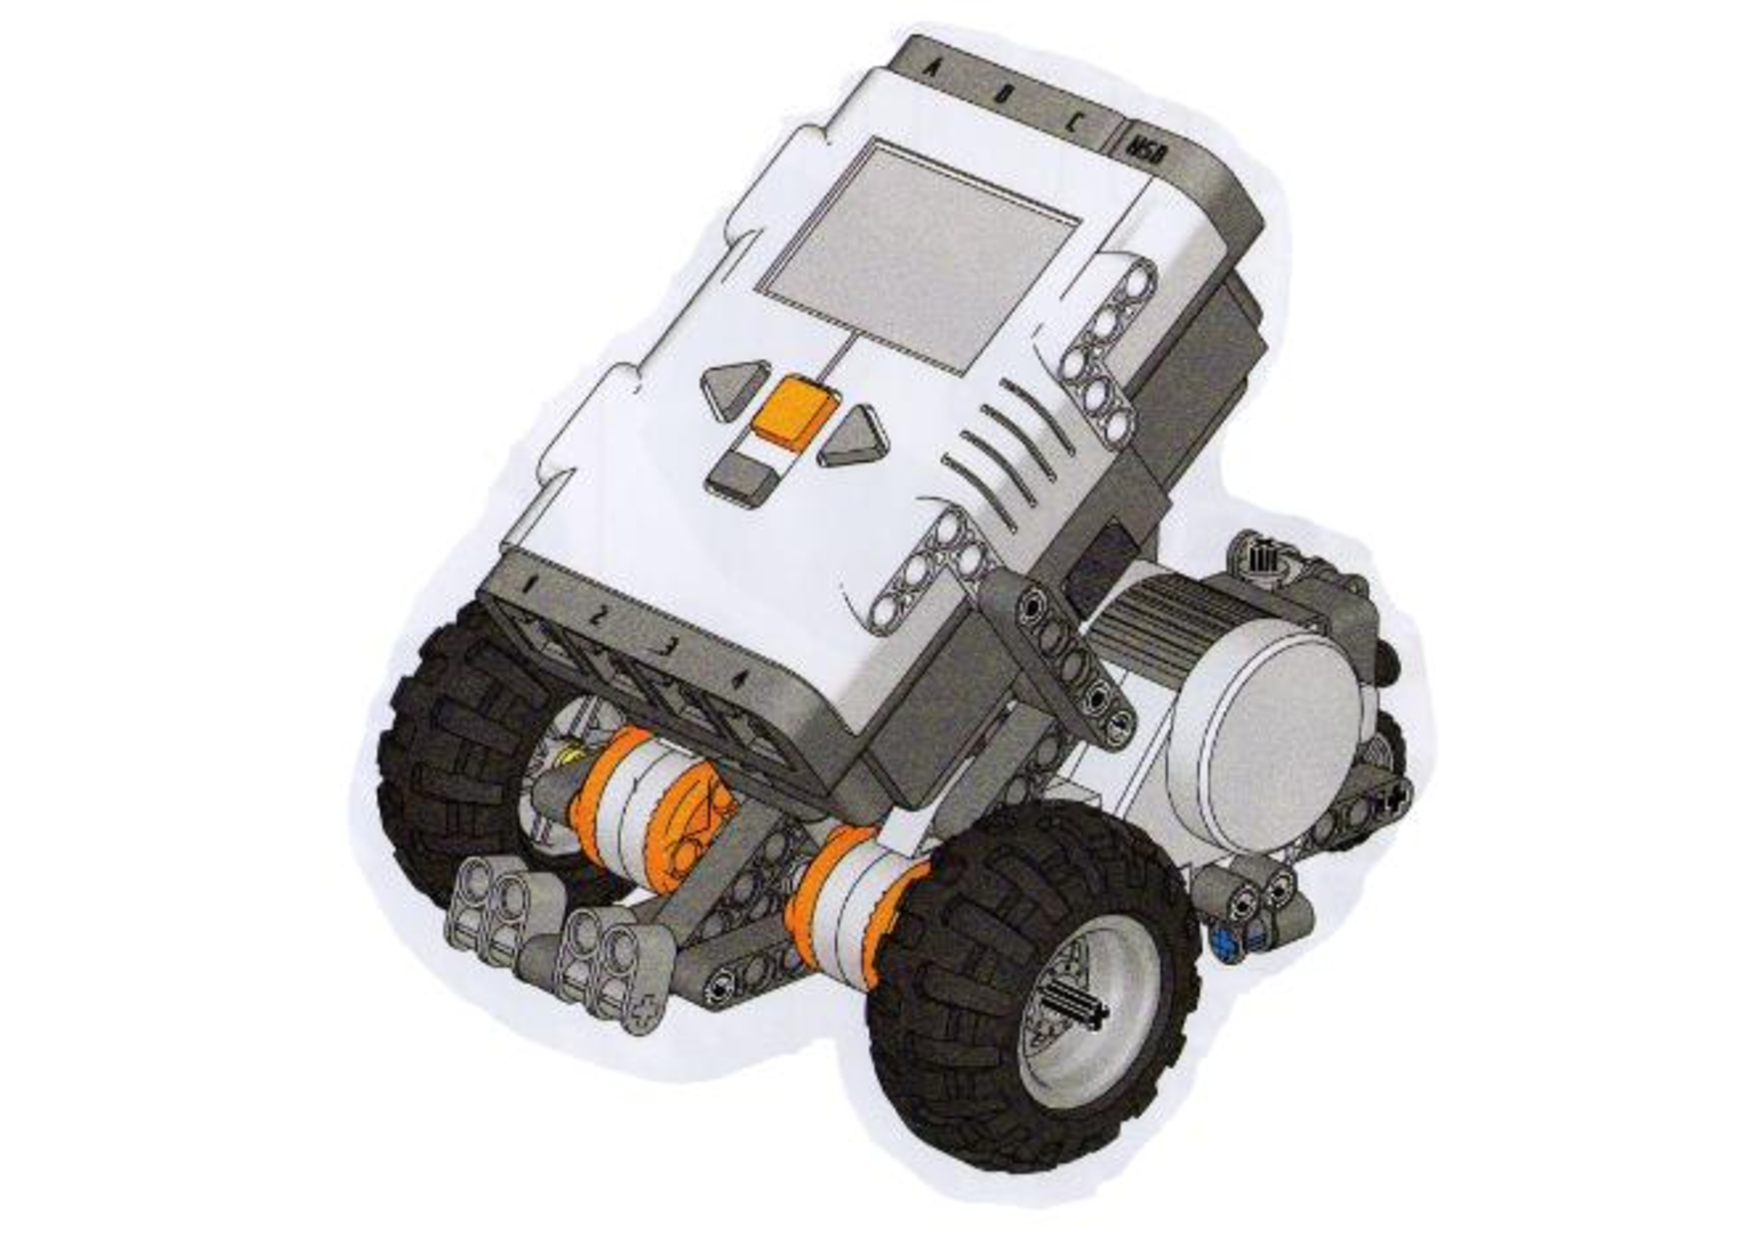
\includegraphics[width=10cm]{./04-figuras/robo}
	\caption{Modelo do Robô}
	\label{fig:robo}
\end{figure}

Após feita a modelagem do problema, foram feitas as implementações e os testes, onde seria possível observar se a odometria feita seria suficiente para alimentar o sistema com precisão e tornar a solução viável. Levando-se em consideração que para tanto foram utilizados os \emph{encoders} óticos acoplados aos motores do \emph{kit Lego Mindstorms\textregistered} que, por sua vez, possuem uma imprecisão que é da ordem de $\pm$ 1 grau por rotação 

Concomitantemente, foram realizadas simulações, através da ferramenta \emph{MATLAB\textregistered}, a fim de prever e validar a modelagem feita do problema, desconsiderando os problemas práticos como, falha na comunicação e falta de sincronismo entre os robôs, erros dos \emph{encoders} e problemas como saturação do motor e derrapagem das rodas. Bem como fazer uma comparação entre o modelo real e o modelo idealizado do sistema.

\section{Modelo Matemático}
\label{sec:modMatematico}
Para introduzir a dinâmica dos robôs móveis utilizados, inicialmente o robô será considerado como um uniciclo, um elemento pontual. A dinâmica de um robô móvel não-holonômico do tipo uniciclo, desconsiderando a dinâmica, pode ser descrita pelas equações abaixo:

\begin{equation}
\dot{x} = v\cos(\theta) 
\label{eq:posiçãox}
\end{equation}
\begin{equation}
\dot{y} = v\sin(\theta)
\label{eq:posiçãoy}
\end{equation}
\begin{equation}
\dot{\theta} = \omega
\label{eq:posiçãotheta}
\end{equation}

sendo:
\begin{itemize}
	\item ($x$,$y$) as coordenadas da posição do robô no plano cartesiano;
	\item $\theta$ o sentido do robô no plano cartesiano;
	\item $v$ e $\omega$ indicam a velocidade linear e angular do robô, respectivamente.	
\end{itemize}

Derivadas dessas equações, surgem as equações \ref*{eq:posiçãoxreal},\ref*{eq:posiçãoyreal} e \ref*{eq:posiçãothetareal} modeladas baseadas no robô real, que não é um elemento pontual no espaço e sim, um modelo não holonômico. Elas serão utilizadas para visualizar a trajetória do robô no ambiente \emph{MATLAB\textregistered} e verificar se a trajetória é compatível com o caminho percorrido pelo robô no mundo real. 

Tendo em vista, que a odometria será feita utilizando-se os \emph{encoders} da própria plataforma e o sistema será realimentado com essas medidas, é de extrema importância que a trajetória observada no mundo real e a registrada pelo robô, através das equações e utilizando-se os \emph{encoders}, sejam consideravelmente semelhantes. Caso o contrário, a realimentação do sistema estará incorreta, comprometendo seriamente, e por que não dizer inviabilizando, o controle do sistema. 

\begin{equation}
x_{k+1} = x_{k} + \dfrac{D_{r} + D_{l}}{2}\cos(\theta_{k}) 
\label{eq:posiçãoxreal}
\end{equation}
\begin{equation}
y_{k+1} = y_{k} + \dfrac{D_{r} + D_{l}}{2}\sin(\theta_{k}) 
\label{eq:posiçãoyreal}
\end{equation}
\begin{equation}
\theta_{k+1} = \theta_{k} + \dfrac{D_{r} - D_{l}}{L}
\label{eq:posiçãothetareal}
\end{equation}

sendo:
\begin{itemize}
	\item $x_{k+1}$ e $x_{k}$ a coordenada $x$ do robô no instante $k$ e no instante $k+1$;
	\item $y_{k+1}$ e $y_{k}$ a coordenada $y$ do robô no instante $k$ e no instante $k+1$;
	\item $\theta_{k+1}$ e $\theta_{k}$ o sentido do robô no instante $k$ e no instante $k+1$;	
	\item $D_{r}$ e $D_{l}$ a distância que a roda direita e esquerda percorreram no instante de tempo entre $k$ e $k+1$, respectivamente;
	\item $L$ o tamanho do eixo do robô;
\end{itemize}

Dado que a velocidade linear e angular de um robô como o do modelo utilizado neste trabalho é dada pela velocidade angular de cada uma das suas rodas unidirecionais, tem-se nas equações \ref{eq:vConv} e \ref{eq:wConv} a função que descreve a velocidade linear e angular do robô baseado na velocidade angular de suas rodas.

\begin{equation}
v = \dfrac{(\omega_{r} + \omega_{l}) rp}{2}
\label{eq:vConv}
\end{equation}
\begin{equation}
\omega = \dfrac{(\omega_{r} - \omega_{l}) rp}{L}
\label{eq:wConv}
\end{equation}

Em que:
\begin{itemize}
	\item $v$ é a velocidade linear do robô;
	\item $\omega$ é a velocidade angular do robô;
	\item $\omega_{r}$ é a velocidade angular da roda direita do robô;
	\item $\omega_{l}$ é a velocidade angular da roda esquerda do robô;
	\item $rp$ é o raio da roda do robô;
	\item $L$ é a distância entre as rodas unidirecionais do robô.
\end{itemize}

\section{Problema 1: \emph{In line}}
\label{sec:P1}
%Reescrever
O primeiro problema consiste em: dado uma frota de \emph{N} robôs, esses robôs devem se alinhar horizontalmente e seguir em linha reta, andando paralelamente, utilizando a estrutura já citada na seção \ref{sec:controleFormacao}, denominada \emph{"In Line"}. Primeiro, este problema será modelado considerando uma modelagem mais simples que será melhor descrita a seguir. 

Considerando-se \emph{N} robôs separados por uma distância $\Delta$$y$ no eixo $y$, cada um em um ponto distinto no eixo $x$, como mostrado na \autoref{fig:p1} (a), a tropa deve se alinhar paralelamente e seguir andando paralelamente com uma velocidade $v_{d}$ constante.

\begin{figure}[!htb]
	\centering
	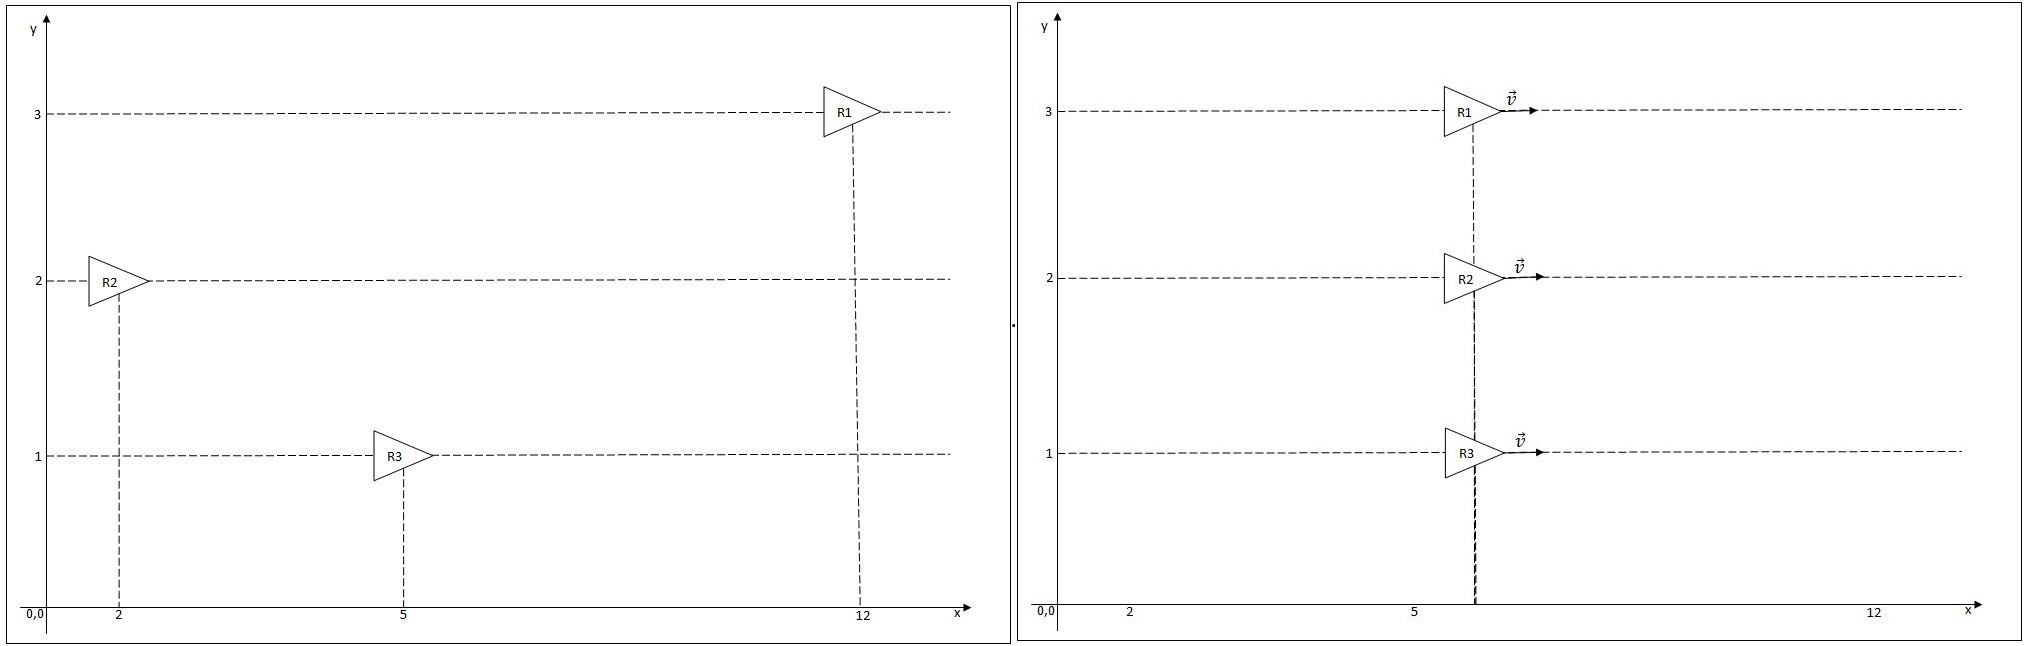
\includegraphics[width=16cm]{./04-figuras/p1}
	\caption{Problema 1: Fig.(a): Sistema no instante i. Fig.(b): Sistema no instante i+k.}
	\label{fig:p1}
\end{figure}

Supondo uma tropa de três robôs, orientados todos no mesmo sentido do eixo x, as velocidades de cada robô devem variar de acordo com o erro de posicionamento do mesmo no eixo x, conforme a distância entre os robôs. Conforme mostrado nas  equações \ref{eq:vel1P1}, \ref{eq:vel2P1} e \ref{eq:vel3P1}. Essas equações fazem com que o robô mais adiantado da frota, imprima uma velocidade menor que os outros robôs, tendendo a se aproximar dos mesmos, em contrapartida os robôs que estão "atrasados" imprimem uma velocidade maior, até que o erro entre eles seja zero e os mesmos caminhem com velocidade constante. 

\begin{equation}
v_{Robo1} = v_{d} + k \times erro_{2,1}
\label{eq:vel1P1}
\end{equation}
\begin{equation}
v_{Robo2} = v_{d} + k\times (erro_{1,2} + erro_{3,2})
\label{eq:vel2P1}
\end{equation}
\begin{equation}
v_{Robo3} = v_{d} + k\times erro_{1,3}
\label{eq:vel3P1}
\end{equation}

Onde,
\begin{itemize}
	\item $v_{Robo1}$, $v_{Robo2}$ e $v_{Robo3}$ são as velocidades que cada robô deve possuir para assumir a formação \emph{in line};
	\item $v_{d}$ é a velocidade que a frota deve assumir após estar alinhada;
	\item $k$ é a constante de ganho proporcional do controlador;
	\item E as variáveis de erro são calculadas, obtendo se a diferença entre a posição no eixo $x$ entre os robôs, como demonstrado na \autoref{eq:errp1}.	
\end{itemize}

\begin{equation}
erro_{i,j} = x_{i} - x_{j}
\label{eq:errp1}
\end{equation}

É importante notar que ao abordar o problemas desta maneira elimina-se o problema de colisão entre os robôs, que estão inicialmente separados no eixo y e alinhados no mesmo sentido, e assim seguem, visto que os mesmos não imprimem velocidade angular. Desta forma, tornando o problema bem didático para ser abordado inicialmente. Posteriormente, será mostrado o problema sendo abordado de outra forma.

\section{Problema 2: Rodeando um alvo}

%O segundo problema consistem em dado um alvo de posiçao $(x,y)$ no plano, a frota deve se locomover até o alvo e o circular, mantendo uma distância $R$ do alvo, com determinada velocidade angular que deve variar de acordo com o tamanho da frota.  

O segundo problema consiste em guiar uma frota de robôs a localizar e circundar, a uma distância \emph{R}, um alvo localizado em uma determinada posição (\emph{x,y}) do plano. E tem como objetivo secundário, ajustar a formação da tropa de robôs que deve se reajustar de acordo com o tamanho da frota, para que continue cobrindo com eficiência a fronteira. Ou seja, caso um ou mais robôs saiam da rede, a frota ira se reajustar para que cada robô tenha a mesma distância entre si e assim, não fique uma grande parte da fronteira sem cobertura, como demostrado na \autoref{fig:sistema}. Que representa uma frota de quatro robôs andando ao redor do alvo, quando então, um dos robôs falha. E o sistema se reajusta para adaptar-se à rede de apenas três robôs.

\begin{figure}[!htb]
	\centering
	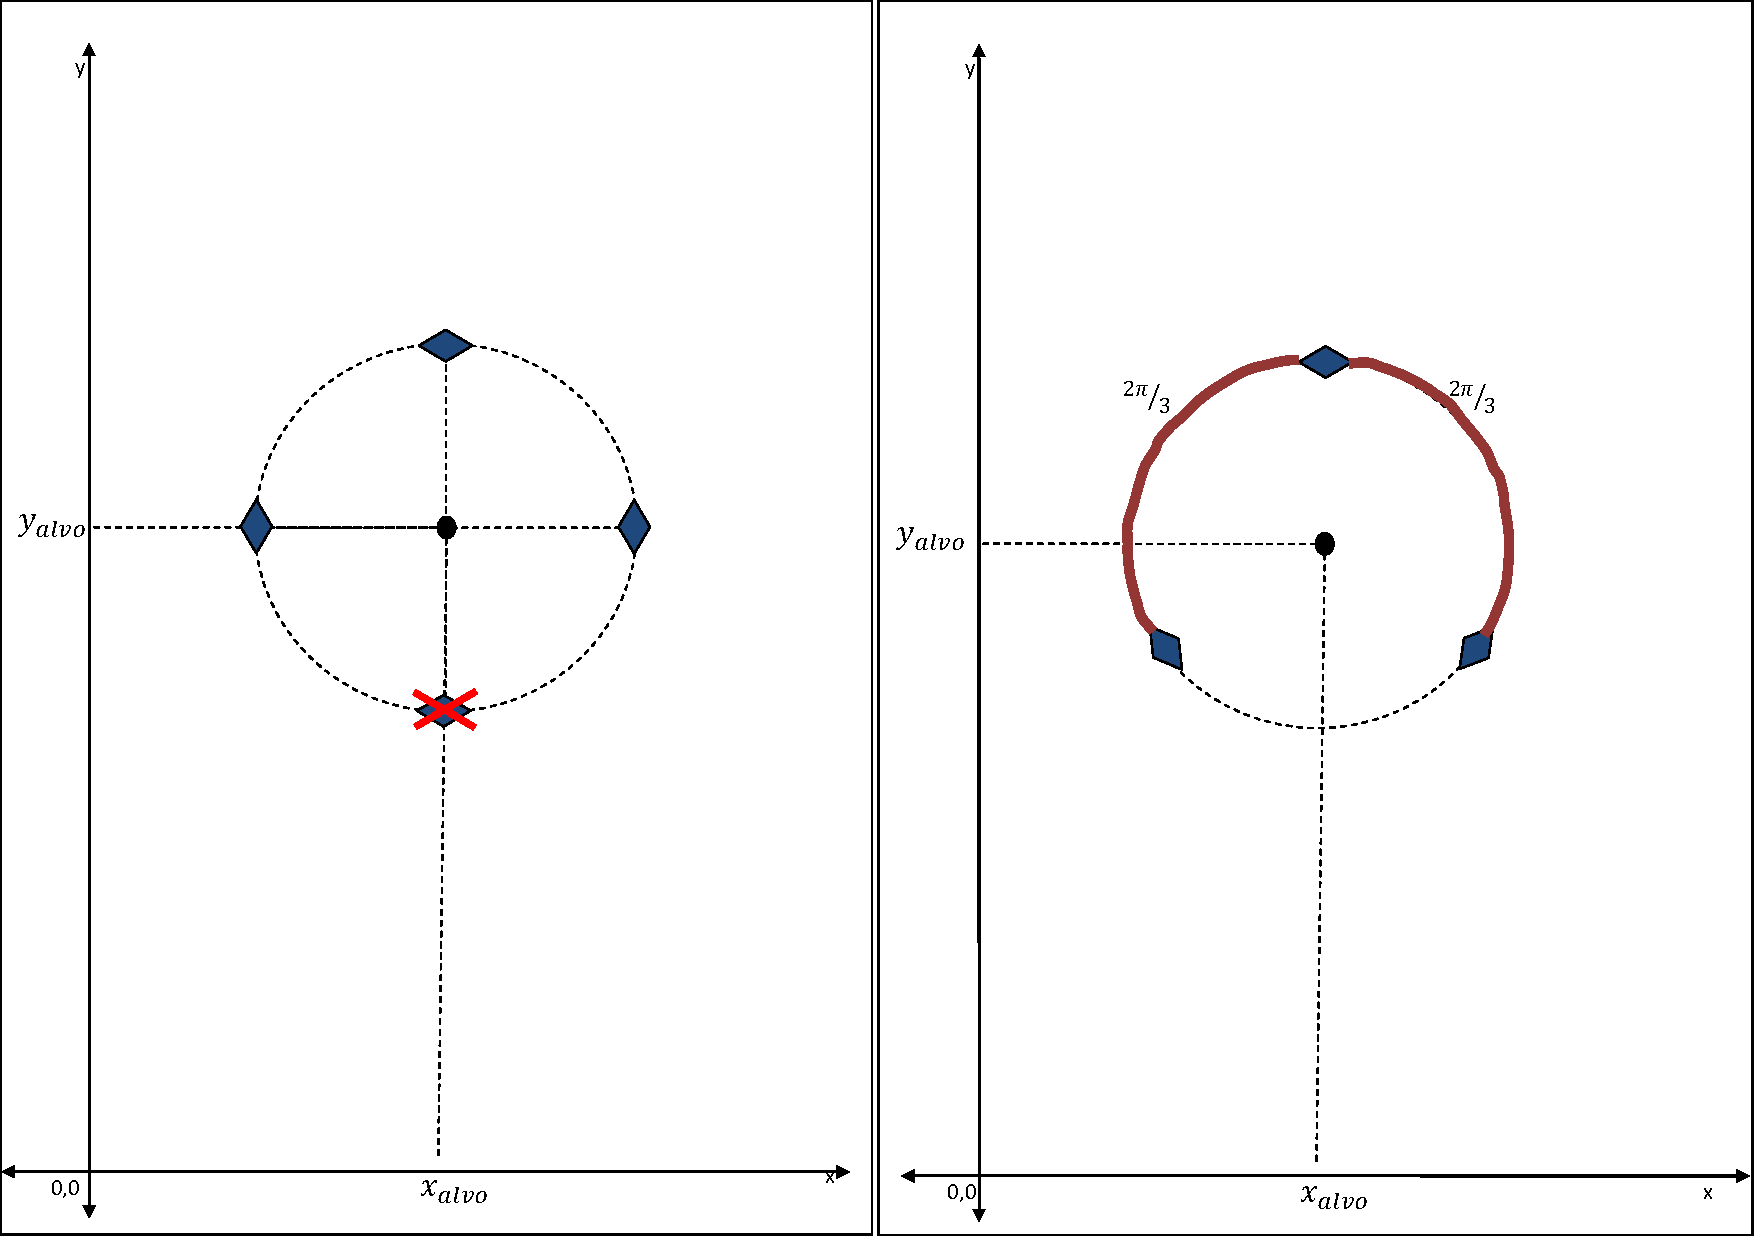
\includegraphics[width=1.0\textwidth]{./04-figuras/sistema}
	\caption{Modelagem do Sistema}
	\label{fig:sistema}
\end{figure}
           % Metodologia
    %
% Documento: Abordagem e modelagem do Problema
%

\chapter{Abordagem e Modelagem do Problema: Malhas de Controle}
\label{chap:abordagememdelo}
%Existem diversas maneiras de se implementar um sistema como este, tanto do ponto de vista do sistema distribuído e sua rede de comunicação, quanto do ponto de vista de controle e realimentação das malhas. Neste capítulo faz-se um detalhamento da abordagem do problema, do funcionamento do sistema como um todo e a modelagem escolhida para abordar os problemas. 

%Para resolução deste problema, primeiramente, estudou-se as possibilidades da implementação do mesmo em uma rede descentralizada, onde não tem-se um mestre definido, apenas uma sociedade de robôs que conforme precisam executar uma tarefa, vão recrutando e formando uma frota. No entanto, concluiu-se que, apesar de viável, a implementação de um sistema distribuído descentralizado seria muito complexo para ser abordado no período deste trabalho, que tem como objetivo principal o estudo de estratégias de controle de formação de múltiplos robôs móveis. Para tanto, foi adotada uma estrutura de rede centralizada denominada 'Mestre/Escravo' e um controle em cascata, utilizado para modularizar o problema e assim, tornar mais simples a implementação e o entendimento do mesmo. 

%Como citado no \autoref{chap:Metod}, serão utilizadas duas abordagens diferentes, uma para resolver apenas o primeiro problema e a outra uma abordagem mais genérica que permite adaptação para resolução de ambos os problemas. A primeira abordagem, utilizará uma malha de controle de velocidade e uma malha de controle que será responsável pela comunicação entre os robôs e definirá a velocidade de cada robô, baseado na posição dos outros integrantes da frota.

%Já a segunda abordagem
Como já dito no \autoref{chap:Metod}, foi escolhida uma estratégia que atende à resolução de ambos os problemas\ a qual, consiste em três malhas de controle: a primeira e mais interna será responsável pelo controle da velocidade angular de cada roda, para se chegar à posição (\emph{x,y}) desejada; a segunda, malha intermediária, será responsável para que cada robô chegue à um determinado ponto (\emph{x,y}) no espaço, portanto, será responsável por corrigir o posicionamento do robô (A primeira e a segunda malhas serão implementadas em cada um dos robôs da frota); a terceira malha e, portanto, a mais externa, é responsável pela coordenação da frota, fornecendo a cada robô as informações necessárias para que o mesmo saiba o ponto (\emph{x,y}) que deve rastrear para consolidar e manter a formação.

Faz-se então neste capítulo um detalhamento das malhas de controle utilizadas e das modificações realizadas para que a estratégia atenda a ambos os problemas, bem como uma descrição de como funcionam as malhas responsáveis pela comunicação e pelo controle de formação para a resolução de cada um dos problemas. Faz-se também um levantamento dos possíveis problemas que podem surgir na implementação do sistema.   
%Faz-se então neste capítulo, primeiramente, a modelagem do problema, para que então, possa-se simular e implementar o problema. Para estabelecer o modelo matemático do problema, será considerado o modelo de robô mostrado na \autoref{fig:robo}.

\section{Malha de Controle 1: Velocidade Angular das Rodas}
\label{sec:malha1 } 
Como já dito anteriormente, este sistema de controle consiste em um controle de três malhas, e agora será abordada a primeira malha. Ela controla os motores para atingir a velocidade angular desejada de cada roda ($\omega_{dr},\omega_{dl}$). Ou seja, a malha de controle vai receber a velocidade linear e angular que se deseja imprimir no robô e retornar a "potência" que deve ser aplicada a cada um dos motores para se atingir as velocidades desejadas, como pode ser observado na \autoref{fig:malha1}.

\begin{figure}[!htb]
	\centering
	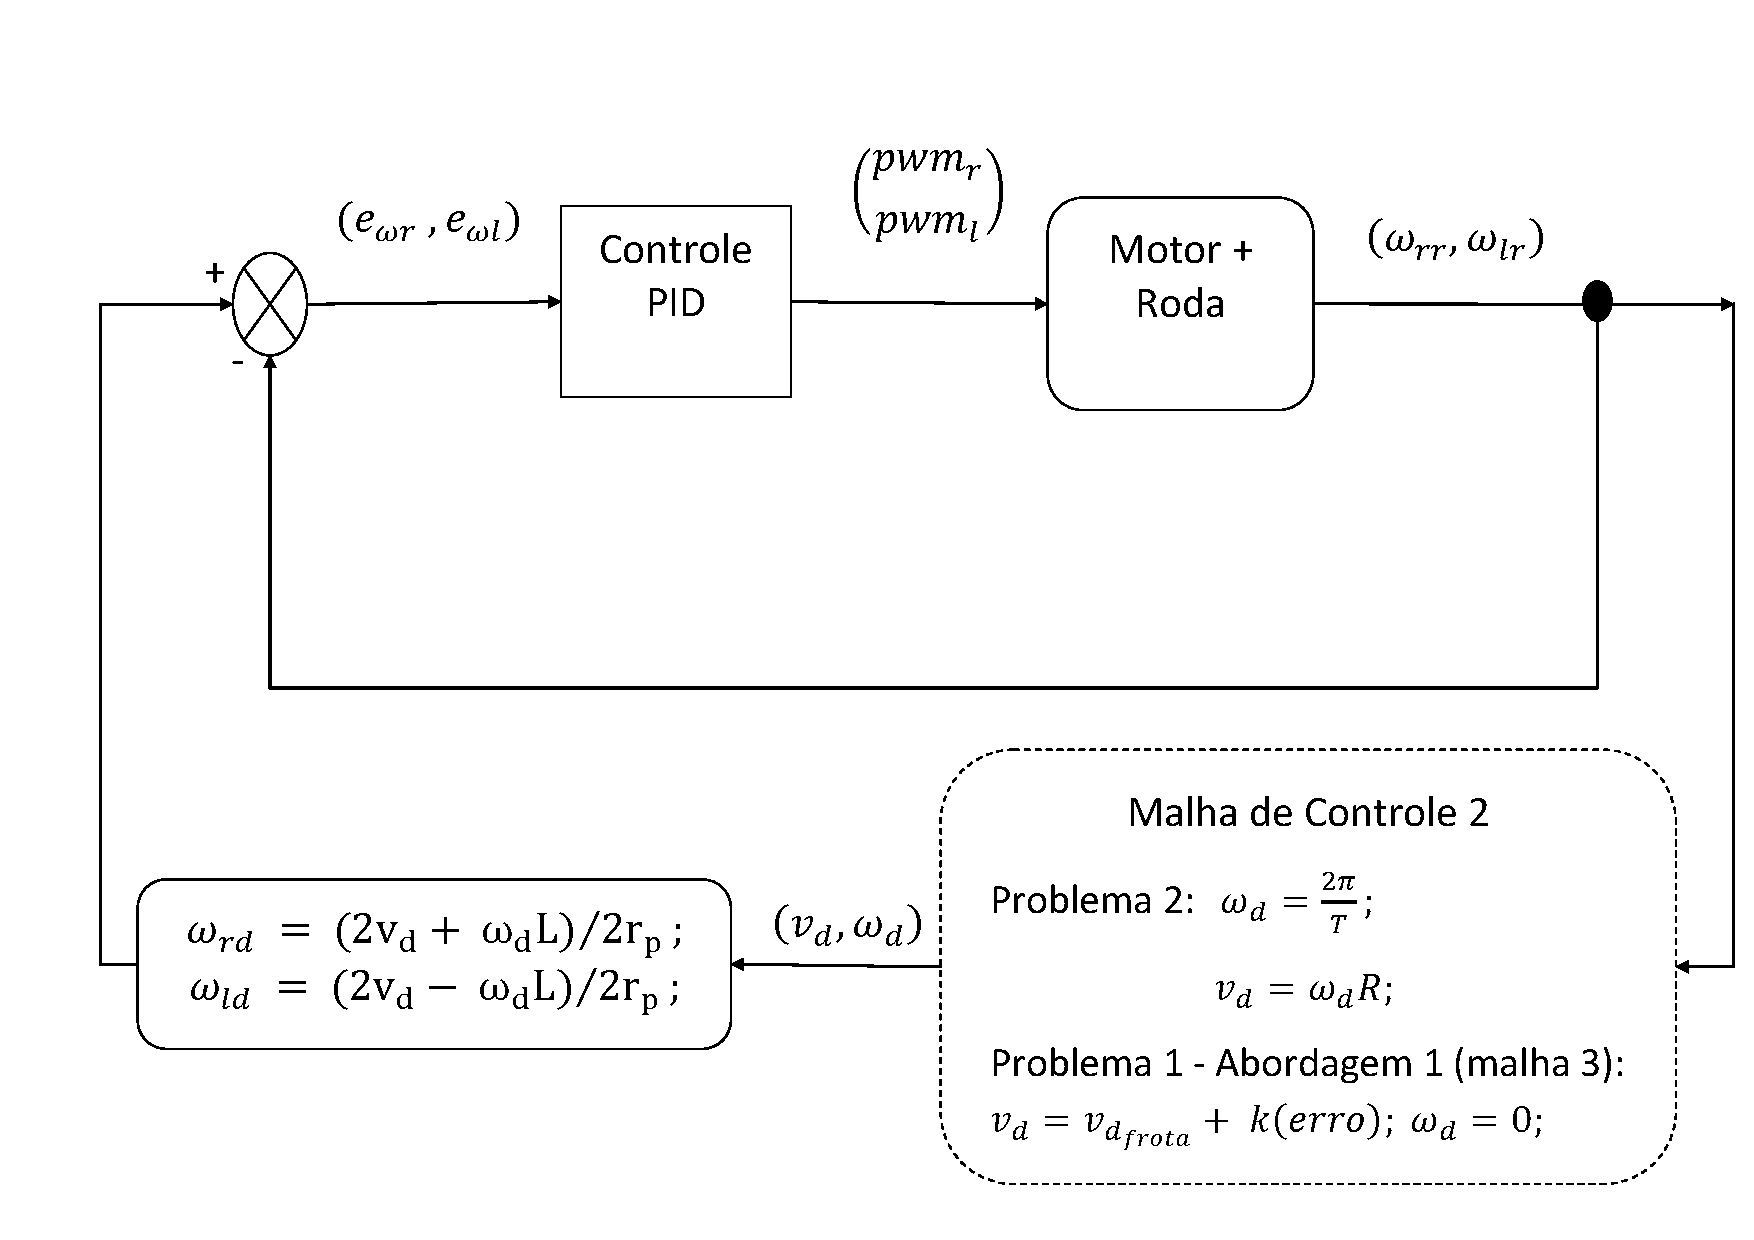
\includegraphics[width=1.0\textwidth]{./04-figuras/malha1}
	\caption{Primeira malha de Controle do Sistema - Controle da velocidade angular}
	\label{fig:malha1}
\end{figure}

É importante ressaltar que como o robô não é um elemento pontual\footnote{Veja a \autoref{fig:sistEst} para visualizá-lo como um elemento não pontual, que depende da variação de velocidade de cada roda para definir a velocidade e o sentido do robô.}, como considerado na \autoref{sec:modMatematico} ao descrever as equações do modelo, temos que descrever a velocidade angular (\emph{$\omega$}) e linear (\emph{$v$}) do robô em função de cada roda, para sabermos a potência a ser aplicada em cada uma delas para que o robô obtenha a velocidade e o sentido desejados.

A partir daí o %módulo 
microcomputador embarcado calcula a velocidade angular desejada de cada roda, como indicado nas equações abaixo que, por sua vez, são oriundas das equações (\ref{eq:vConv}) e (\ref{eq:wConv}):
\begin{subequations}
\begin{equation}
\omega_{dr} = \dfrac{2v + \omega_{d}L}{2r_{p}}	
\label{eq:velocangulardireita}
\end{equation} 
\begin{equation}
\omega_{dl} = \dfrac{2v - \omega_{d}L}{2r_{p}}	
\label{eq:velocangularesquerda}
\end{equation} 
\label{eq:convVelAngRodas}
\end{subequations}
onde:
\begin{itemize}
	\item $v_d$ é a velocidade linear desejada do robô ($m/s$);
	\item $\omega_{dr}$ é a velocidade angular desejada da roda direita ($rad/s$);
	\item $\omega_{dl}$ é a velocidade angular desejada da roda esquerda ($rad/s$);
	\item $r_{p}$ o raio da roda ($m$);
	\item $L$ o tamanho do eixo das rodas do robô ($m$).	
\end{itemize}

Com a velocidade angular de cada roda  do robô, estimada a partir dos dados fornecidos pelos \emph{encoders}, é calculado o erro das velocidades dado por:%, como mostrado nas equações abaixo, 
\begin{equation}
e_{wr} = \omega_{dr} - \omega_{rr}
\label{eq:errVelAngDireita}
\end{equation} 
\begin{equation}
e_{wl} = \omega_{dl} - \omega_{rl}
\label{eq:errVelAngEsquerda}
\end{equation} 
onde:
\begin{itemize}
	\item $e_{wr}$ e $e_{wl}$ são os erros da velocidade angular da roda direita e esquerda, respectivamente;
	\item $\omega_{rr}$ e $\omega_{rl}$ é a velocidade angular real da roda direita e esquerda, respectivamente.
\end{itemize}
E o controlador os retorna as ações de controle que serão passadas como potência para cada uma das rodas.	

\section{Malha de Controle 2: Posicionamento}
\label{sec:malha2 } 
Para que a malha de controle 3, que consiste no controle de formação do sistema multiagente funcione, primeiramente é necessário implementar o controle de posicionamento de cada robô. Ou seja, para que o robô cumpra a missão, é necessário que a malha de controle de formação passe para cada robô os parâmetros necessários para o ajuste da estrutura, tais como, posicionamento, velocidade e número de robôs da frota. Cada robô por sua vez, deve conseguir se posicionar corretamente de acordo com a posição recebida pela malha de controle 3, o que só será possível se a malha de controle 1 conseguir controlar adequadamente os motores para que eles imprimam a velocidade correta em cada roda.

Como pode ser visto na \autoref{fig:esq2}, o problema a ser resolvido pela segunda malha de controle consiste em, dado um sistema de coordenadas cartesianas, onde têm-se um robô móvel de posição (\emph{$x_{r},y_{r}$}), cuja orientação (\emph{$\theta$}) é indicada em relação ao eixo \emph{x} do sistema, %onde pretende-se 
fazer com que o robô chegue ao ponto desejado (\emph{$x_{d},y_{d}$}), recebido da malha de controle 3. Para tanto, a malha 2 funciona da seguinte maneira: Recebe da malha 3 os parâmetros necessários para o cálculo da posição desejada do robô (\emph{$x_{d},y_{d}$}), e a partir daí é determinado o erro de posição do robô (\emph{$e_{x},e_{y}$}), fazendo-se a diferença entre a posição desejada e a posição real do robô (\emph{$x_{r},y_{r}$}), que é obtida através dos \emph{encoders} do LEGO\textregistered, que se mostrou suficientemente precisos.

\begin{equation}
e_{r} = r_{d} - r_{r}
\label{eq:errr}
\end{equation}
\begin{equation}
e_{x} = x_{d} - x_{r}
\label{eq:errx}
\end{equation}
\begin{equation}
e_{y} = y_{d} - y_{r}
\label{eq:erry}
\end{equation}

Através do erro de posicionamento do robô, encontra-se o ângulo de orientação desejado\footnote{Para fins de implementação é altamente recomendável o uso da função \emph{atan2} que mapeia o ângulo de orientação para o intervalo entre $-\pi$ e $\pi$, contemplando todos os quatro quadrantes do plano $xy$. Essa função é utilizada neste trabalho para calcular o ângulo de orientação desejado e limitar o erro do ângulo de orientação.}, dado por: %(\emph{$\theta_{d}$}), como mostrado na \autoref{eq:thetad}. 
\begin{equation}
\theta_{d} = \arctan\left(\dfrac{e_{y}}{e_{x}}\right)
\label{eq:thetad}
\end{equation}
Então, o erro do ângulo de orientação do robô é obtido, através da %\autoref{eq:errtheta} abaixo.
equação indicada abaixo: 
\begin{equation}
e_{\theta} = \theta_{d} - \theta_{r}
\label{eq:errtheta}
\end{equation}

O erro do ângulo de orientação (\emph{$e_{\theta}$}) é passado para o controlador que retorna a velocidade linear e angular da ação de controle, que será passada para a malha mais interna (malha 1). %Posteriormente, será feita uma comparação entre os controladores \emph{PI} e \emph{PID} e será definido o controlador a ser utilizado nesta malha.

\begin{figure}[!htb]
	\centering
	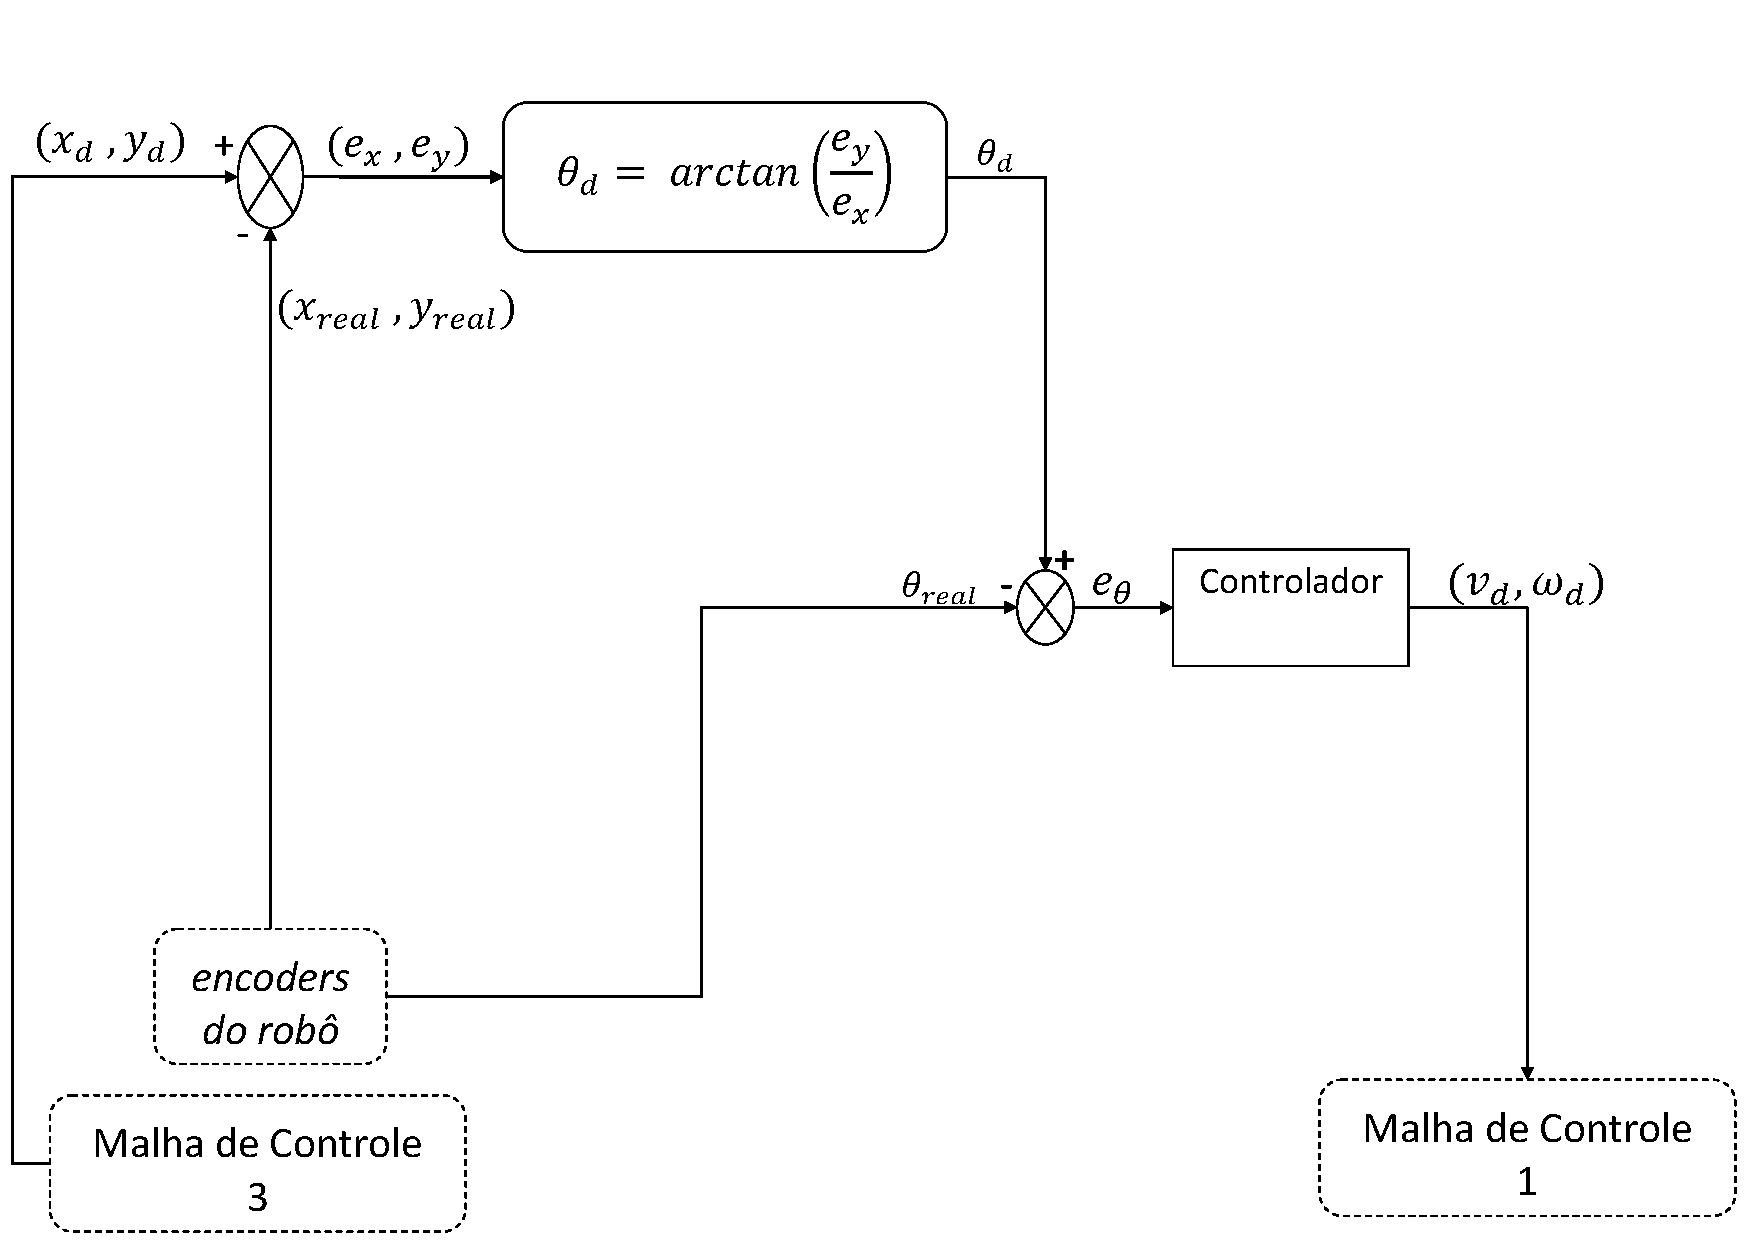
\includegraphics[width=1.0\textwidth]{./04-figuras/malha2}
	\caption{Segunda malha de Controle do Sistema - Controle de Posicionamento}
	\label{fig:malha2}
\end{figure}

\section{Malha de Controle 3: Controle de formação}
\label{sec:malha3 }
A malha de controle de formação tem como função estabelecer a comunicação entre os robôs, enviando os dados necessários para que se estabeleça a formação da frota. Além disso, ela utiliza as informações recebidas para estabelecer a posição em que o robô deve assumir naquele instante. Existem duas formas de se fazer esse controle, uma delas consiste em centralizar este controle de formação no mestre e enviar para o restante da frota apenas a posição desejada já calculada; já a outra consiste na troca de informações entre os agentes do sistema sem sobrecarregar o mestre.

No caso do primeiro problema (varredura de área em paralelo), é necessário que cada robô saiba a posição no eixo das abscissas de todos os outros robôs e a partir daí calcule a posição desejada, ou seja, um determinado robô recebe a posição dos outros robôs da frota e utiliza a \autoref{eq:xdp1} para obter a posição desejada do robô naquele instante, que é passada para a malha de controle intermediária, que por sua vez calcula o erro de posicionamento e envia para a malha de controle de velocidade interna as velocidades que devem ser assumidas pelo robô para que o mesmo possa alcançar a posição desejada e cumprir os objetivos estabelecidos. É importante ressaltar que, a depender da rede implementada, como é o caso deste trabalho em que a rede é centralizada e os robôs escravos não se comunicam entre si, essas informações devem ser passadas de um robô para o outro sempre através do mestre. %entre a frota através do mestre.

Já no caso do segundo problema (circulação de um robô), as informações que cada robô deve possuir para assumir a formação da frota são: número de robôs da frota, numeração que aquele robô representa na frota e posição do alvo. A partir daí é possível utilizar as \autoref{eq:posDesejada_p2} para se obter a posição desejada para que aquele robô contribua positivamente para a formação da estrutura da frota. Como pode ser visto na \autoref{eq:posDesejada_p2}, a definição da posição desejada leva em consideração o tempo, o que é um problema na aplicação prática, visto que não há uma sincronia entre os relógios dos robôs. Dessa forma, para contornar este problema, será levado em consideração o relógio do mestre, sendo necessário que essa variável também seja repassada ao restante da frota. 

%É importante notar que esta malha de controle não é uma malha fechada, ou seja, ela não possui realimentação. Esta malha apenas controla as informações e para quais robôs as mesmas devem ser enviadas, além de calcular a posição desejada utilizando-se das equações já mostradas anteriormente. 







%Ou seja, deseja-se circular o alvo em um período de \emph{T} segundos, a malha de controle de velocidade vai receber a velocidade angular desejada ($ \omega _{d} $), que é uma derivação do período de circulação desejado, como mostrado na equação abaixo:



 

		%Desenho e Modelo do Sistema
    \chapter{Simulações}
\label{chap:Simulacoes}

As simulações realizadas neste trabalho, consideram o robô como um elemento pontual, conforme descrito nas equações \ref{eq:posiçãox}, \ref{eq:posiçãoy} e \ref{eq:posiçãotheta} e foram realizadas com intuito de se observar a viabilidade de implementação da estratégia de controle. 

Essas implementações desconsideram não só o robô como um elemento não-pontual, mas também, desconsideram problemas como: saturação do motor, derrapagem das rodas, falhas de comunicação e imprecisão de leitura dos \emph{encoders}. 

\section{Simulações do Primeiro Problema}
\label{sec:SimulacaoP1}

Primeiramente, foi realizado a simulação da primeira estratégia de abordagem do primeiro problema, em que tem-se uma frota de \emph{N} robôs separados entre si no eixo $y$ e com uma posição randômica no eixo $x$, todos dispostos na mesma direção e sentido. A primeira estratégia elimina os problemas de colisão, visto que os robôs começam separados, no mesmo sentido e como são impossibilitados a imprimir uma velocidade angular pela estratégia adotada, seguem em linha reta com velocidade linear negativa ou positiva. Além disso, ela leva em consideração a rede de comunicação, utilizando-se a \autoref{eq:velP1}. 

Serão feitas simulações com duas redes, a primeira será uma rede centralizada com 4 robôs, tal qual é possível implementar com a plataforma \emph{Lego Mindstorms\textregistered}. A segunda, será uma rede descentralizada com cinco robôs, tal como a rede ilustrada na \autoref{fig:rededistr}. Como mostrado nas Figuras \ref{fig:sP1Cent} e \ref{fig:sP1Desc}, essa é uma estratégia viável quando considerando o robô como um elemento pontual.

\begin{figure}[!htb]
	\centering
	\begin{subfigure}{.5\textwidth}
		\centering
		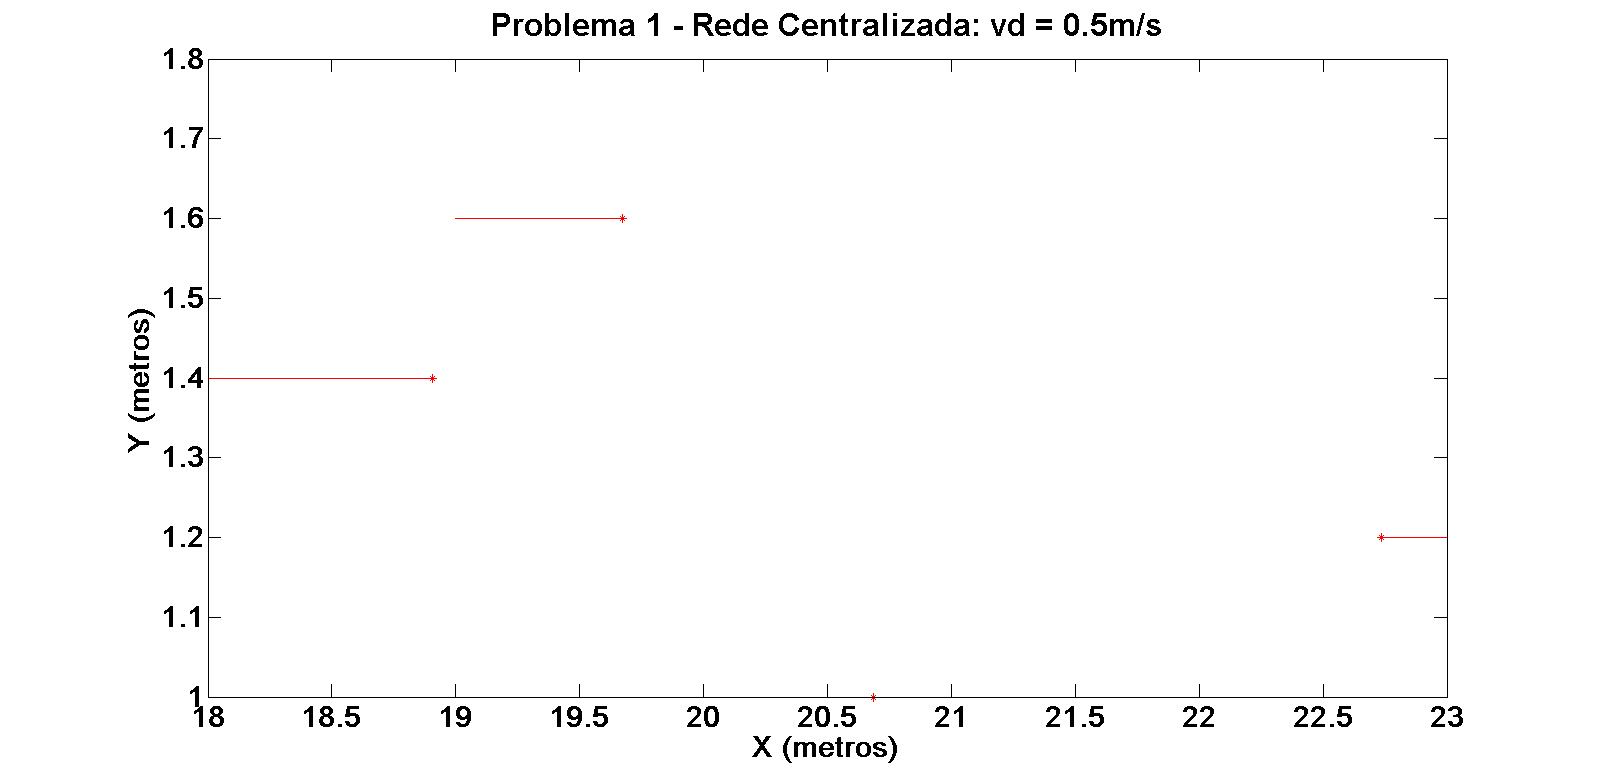
\includegraphics[width=.9\linewidth]{./04-figuras/Simulacoes/Problema1-Abordagem1/P1_A1_Centr_Inicio}
		\caption{Sistema com Rede Centralizada - Antes do alinhamento dos robôs}
		\label{fig:P1CIni}
	\end{subfigure}%
	\begin{subfigure}{.5\textwidth}
		\centering
		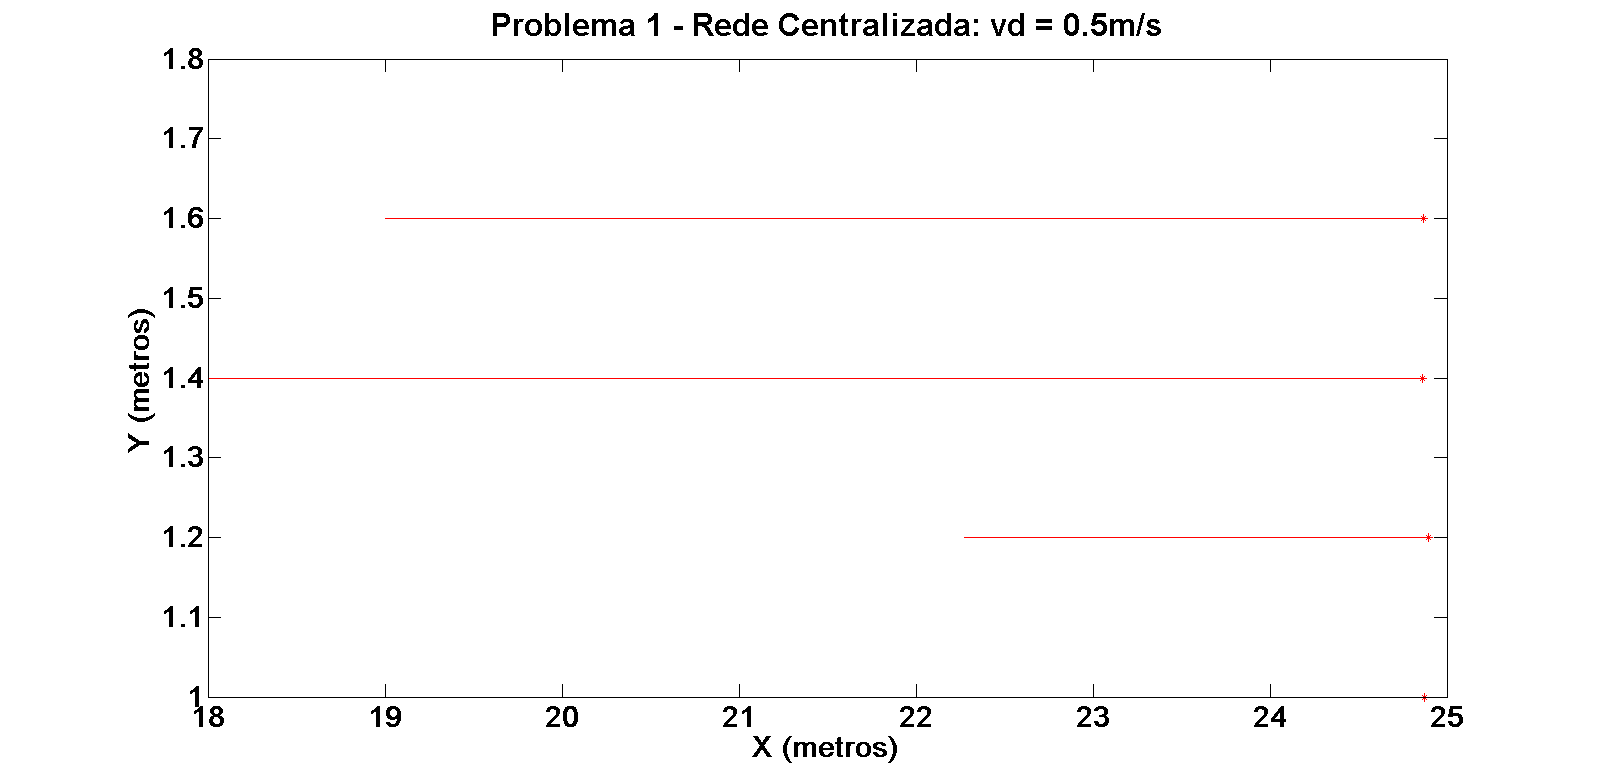
\includegraphics[width=.9\linewidth]{./04-figuras/Simulacoes/Problema1-Abordagem1/P1_A1_Centr_Fim}
		\caption{Sistema com Rede Centralizada - Depois do alinhamento dos robôs}
		\label{fig:P1CFim}
	\end{subfigure}
	\caption{Problema 1 - Primeira Abordagem com Rede Centralizada}
	\label{fig:sP1Cent}
\end{figure}

\begin{figure}[!htb]
	\centering
	\begin{subfigure}{.5\textwidth}
		\centering
		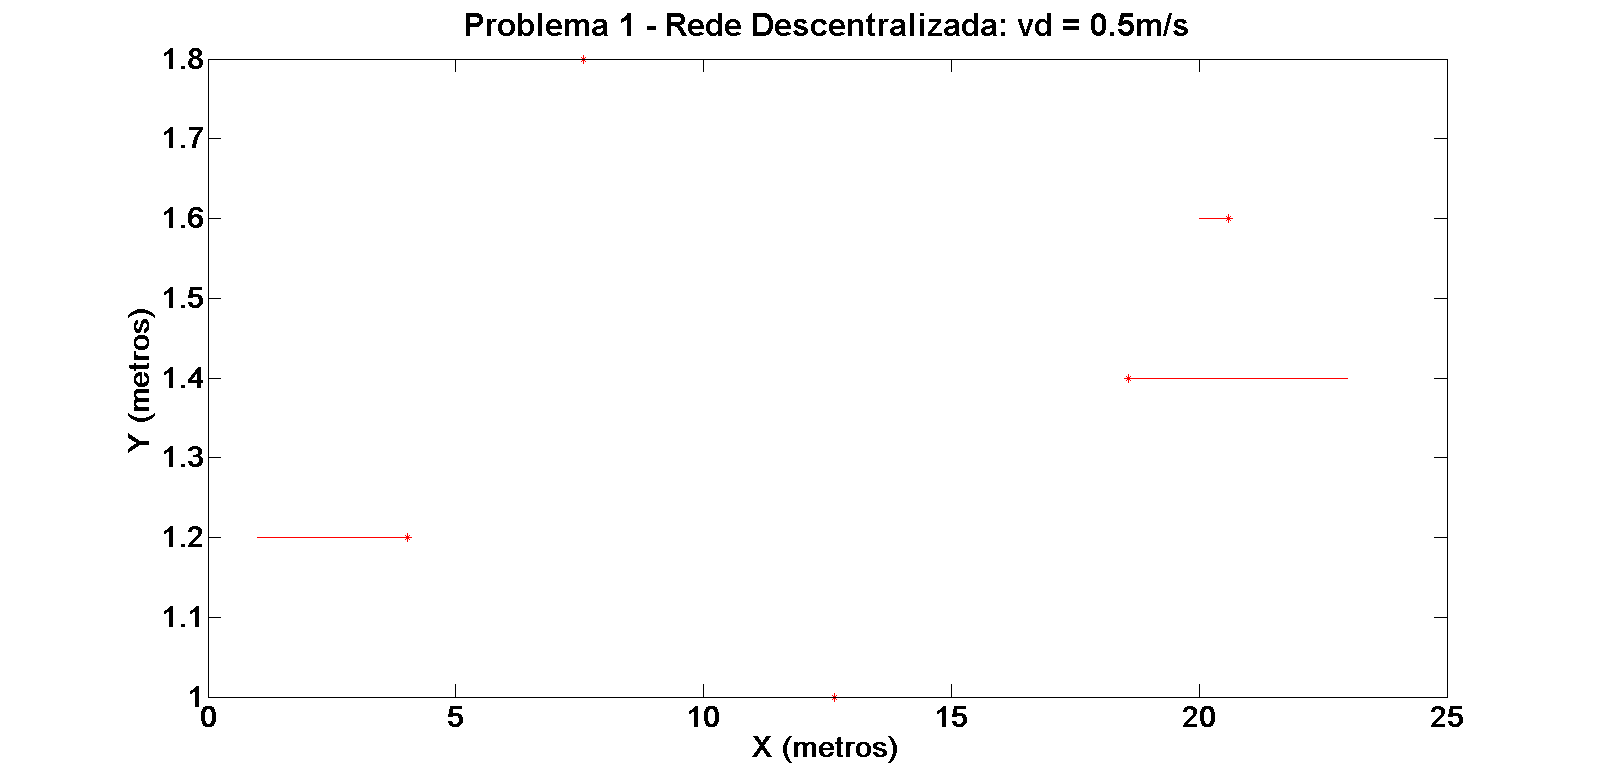
\includegraphics[width=.9\linewidth]{./04-figuras/Simulacoes/Problema1-Abordagem1/P1_A1_Desc_Inicio}
		\caption{Sistema com Rede Descentralizada - Antes do alinhamento dos robôs}
		\label{fig:P1DIni}
	\end{subfigure}%
	\begin{subfigure}{.5\textwidth}
		\centering
		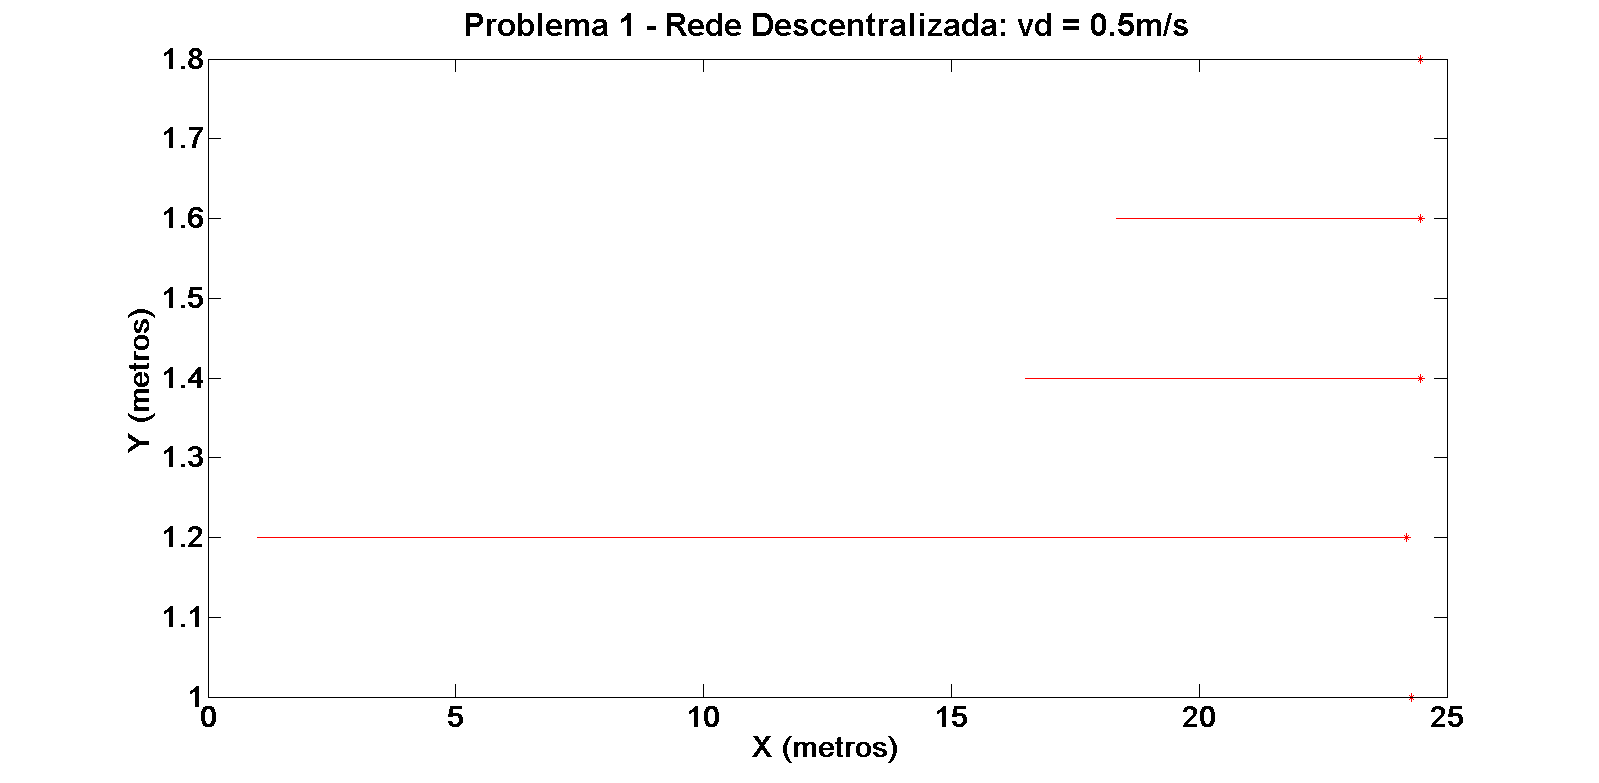
\includegraphics[width=.9\linewidth]{./04-figuras/Simulacoes/Problema1-Abordagem1/P1_A1_Desc_Fim}
		\caption{Sistema com Rede Descentralizada - Depois do alinhamento dos robôs}
		\label{fig:P1DFim}
	\end{subfigure}
	\caption{Problema 1 - Primeira Abordagem com Rede Descentralizada}
	\label{fig:sP1Desc}
\end{figure}

Já a segunda estratégia consiste em encontrar uma reta paralela ao eixo y onde, sua localização no eixo x é a média da posição dos robôs mais distantes entre sí do sistema. Ela foi implementada de modo a permitir que o robô adquirira uma velocidade angular. Sendo assim ele pode se deslocar em qualquer direção. Essa abordagem faz uso da malha de controle intermediário modelada no \autoref{chap:abordagememdelo} e apresenta problemas de colisão, já que os robôs podem se deslocar em qualquer direção.

Não foi implementado neste trabalho um tratamento de colisão, foram adotadas algumas medidas para diminuir as colisões no sistema. A primeira medida foi estabelecer uma prioridade na rede que vai do mestre ao último escravo, aquele que possui menor prioridade para ao estar em menos de 20 centímetros de distância de outro robô. A segunda medida foi fazer com que os robôs convirjam um a um para o ponto desejado. Notou-se com essas medidas uma redução\footnote{Foram realizados 1000 experimentos com 300 amostras cada um, primeiro sem nenhuma medida para evitamento de colisão, depois apenas parando o robô com menor prioridade e por fim, uma combinação entre a segunda técnica e a técnica de convergir os robôs um a um para o ponto desejado. Percebeu-se com isso uma redução de 80\% com aplicação da primeira técnica e de 87\% com a aplicação de ambas as técnicas.} no número de colisões ocorridas no sistema..

Como pode ser visto na \autoref{fig:sP1A2}, essa abordagem também é viável entretanto, apesar de apresentar a vantagem de conceder mais autonomia aos robôs, deixando-os movimentar em qualquer direção, ela acarreta ao sistema problemas de colisão que quando não contornados podem prejudicar o sistema.

\begin{figure}[!htb]
	\centering
	\begin{subfigure}{1.0\textwidth}
		\centering
		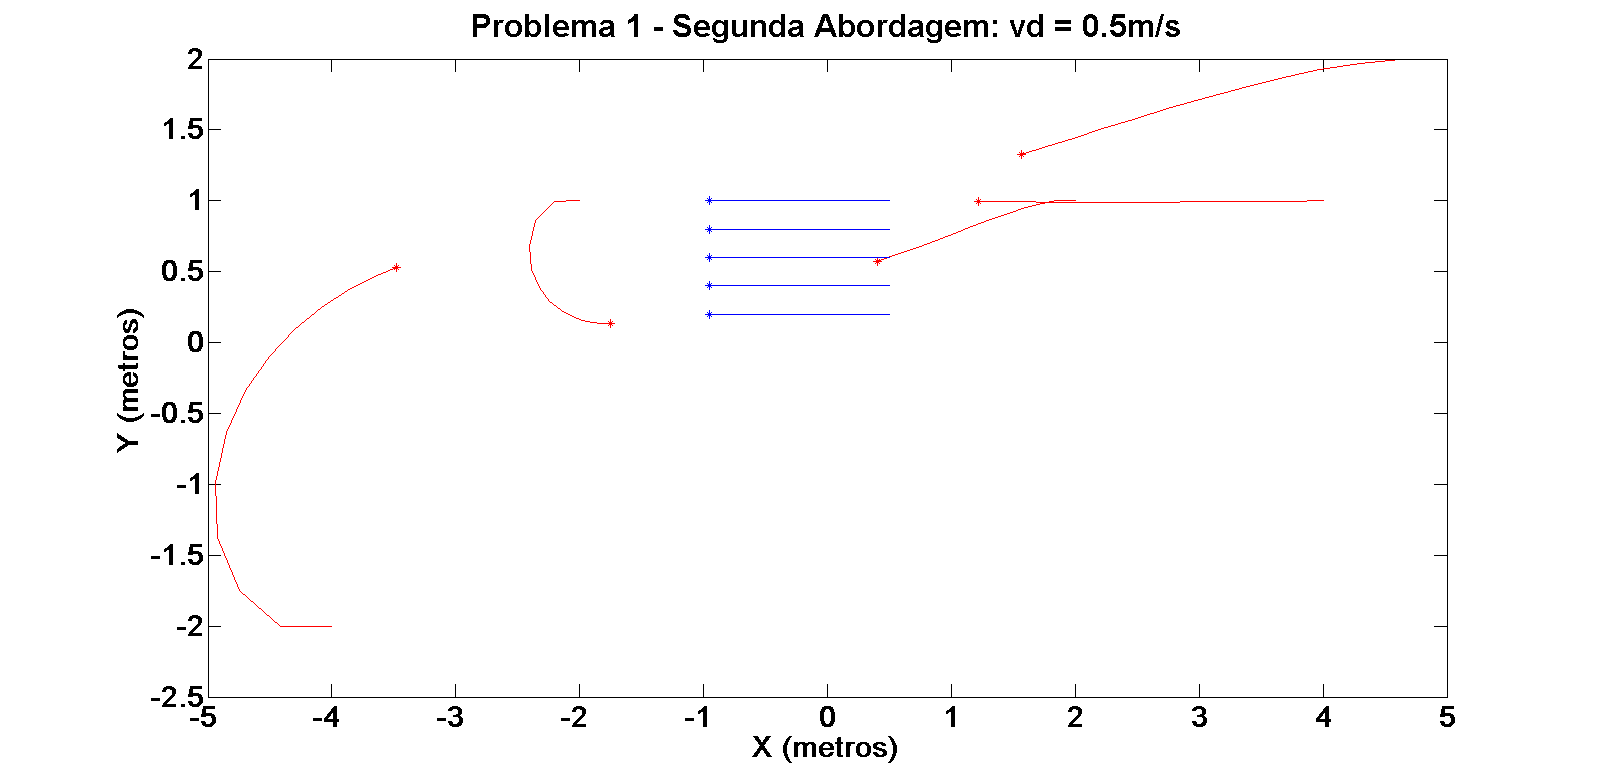
\includegraphics[width=.9\linewidth]{./04-figuras/Simulacoes/Problema1-Abordagem1/P1A2Inicio}
		\caption{Segunda Abordagem - Antes do alinhamento dos robôs}
		\label{fig:P1A2Ini}
	\end{subfigure}
	\begin{subfigure}{1.0\textwidth}
		\centering
		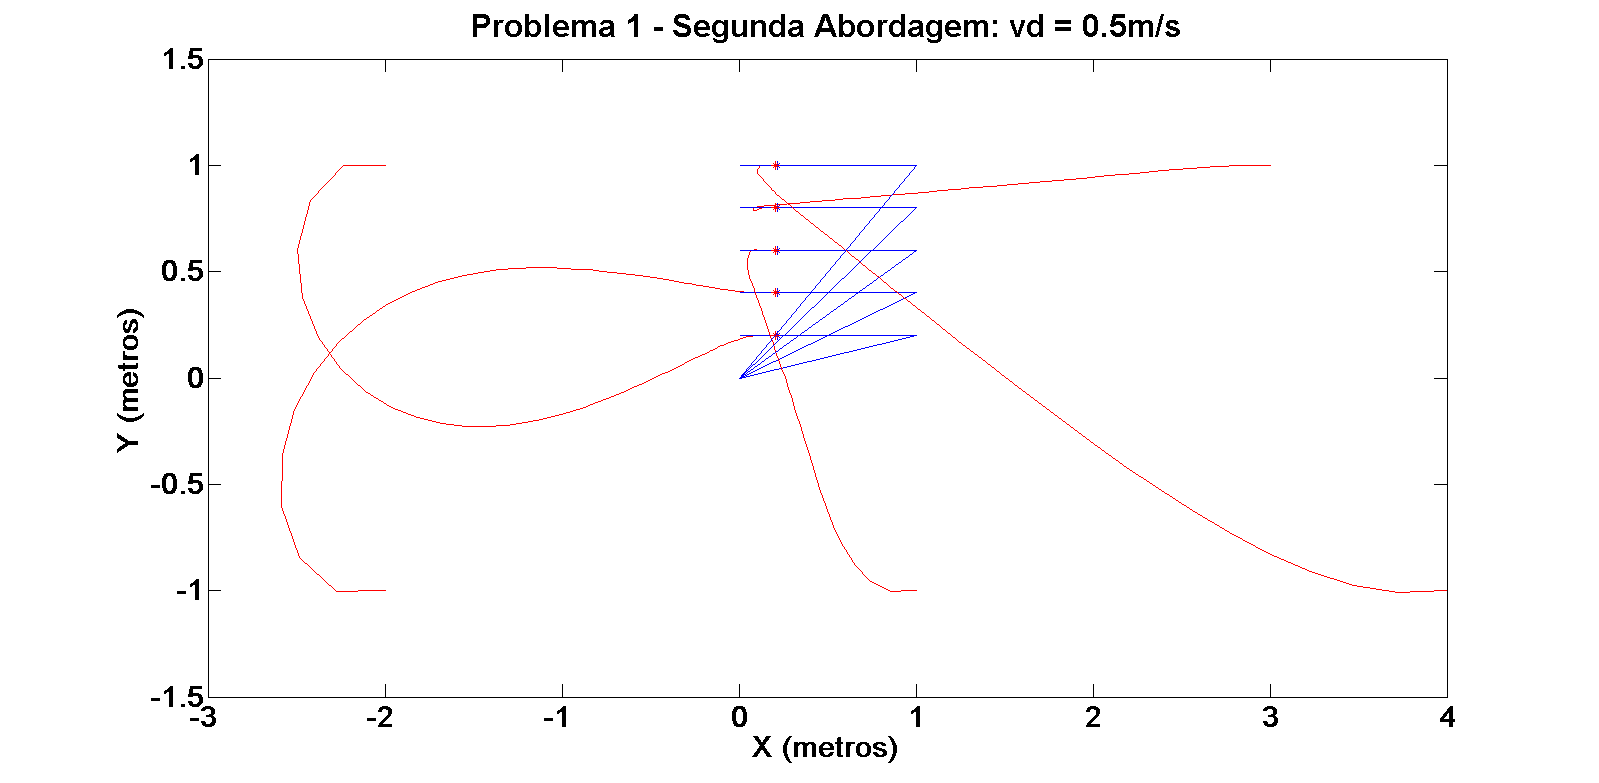
\includegraphics[width=.9\linewidth]{./04-figuras/Simulacoes/Problema1-Abordagem1/P1A2Fim}
		\caption{Segunda Abordagem - Depois do alinhamento dos robôs}
		\label{fig:P1A2Fim}
	\end{subfigure}
	\caption{Problema 1 - Segunda Abordagem}
	\label{fig:sP1A2}
\end{figure}

\section{Simulações do Segundo Problema}
\label{sec:SimulacaoP2}
Como já dito anteriormente neste trabalho, o segundo problema consiste em guiar uma frota de robôs a um determinado alvo e circulá-lo a uma distância \emph{R} e um período \emph{T}. Dito isto, fez-se algumas simulações para validar o modelo matemático e compará-lo ao modelo real. Esta simulação desconsidera um problema enfrentado no mundo real que é a falta de sincronismo entre os relógios dos motores, visto que o tempo corrido em simulação é igual para todos os robôs da frota. 

A primeira simulação realizada desconsidera problemas de colisão e inicia os robôs com posições randômicas. Após mil intervalos de amostragem retiram-se dois robôs e verifica-se que o sistema se reorganiza, mantendo os robôs a mesma distância angular entre si. Já nas simulações seguintes foram tomadas as medidas citadas na \autoref{sec:SimulacaoP1} para evitar que ocorra colisão entre os robôs. Como pode ser visto nas figuras \ref{fig:sP2F}, \ref{fig:P2C}, as estratégias modeladas são viáveis dentro de um ambiente de simulação computacional.%pouco realístico. 

\begin{figure}[!htb]
	\centering
	\begin{subfigure}{1.0\textwidth}
		\centering
		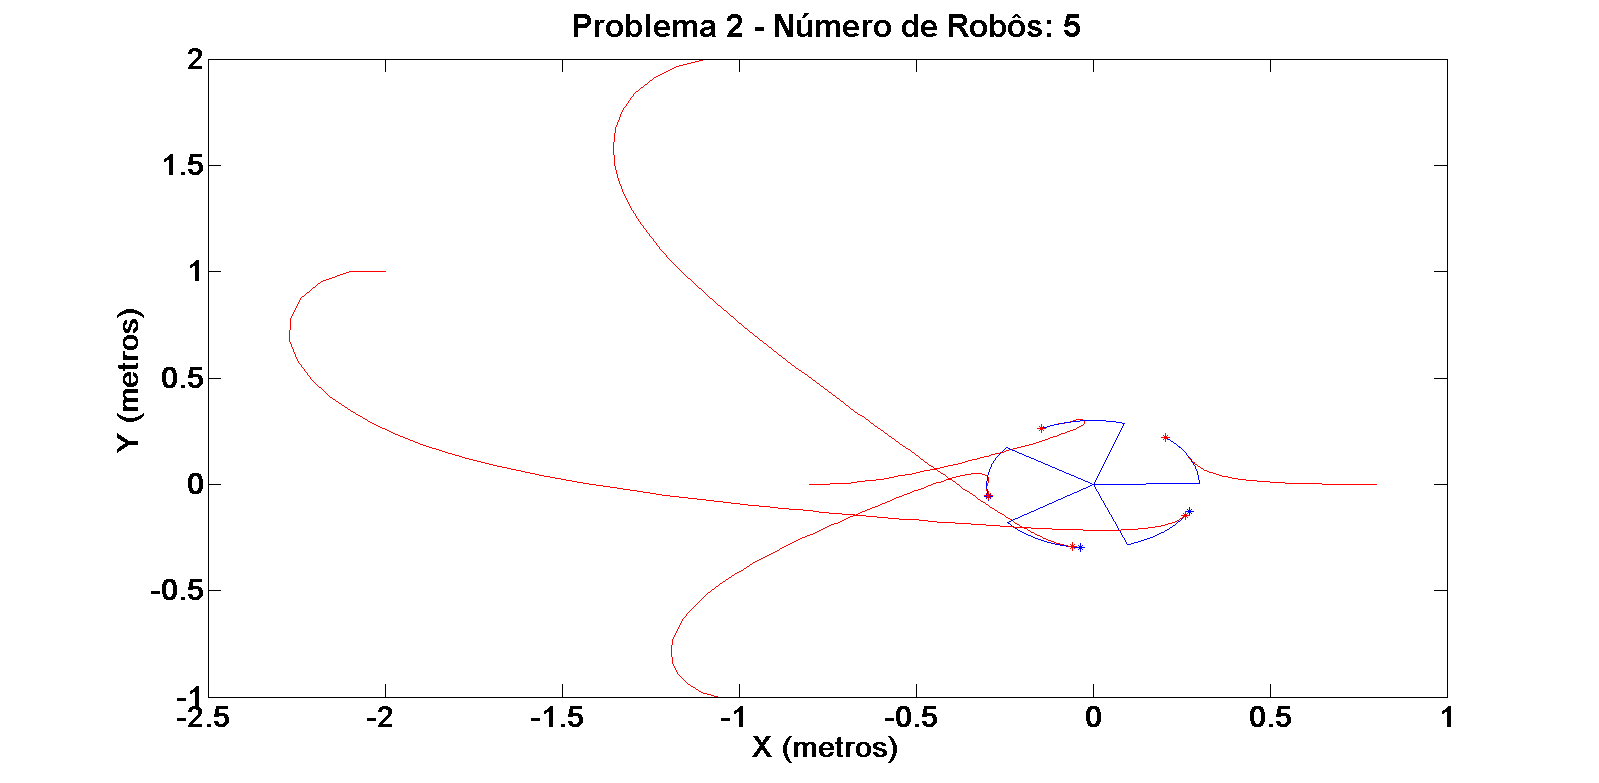
\includegraphics[width=.9\linewidth]{./04-figuras/Simulacoes/Problema2/Falha/P2FalhaInicio}
		\caption{Segundo Problema - Cinco Robôs Alinhados}
		\label{fig:P2SF}
	\end{subfigure}
	\begin{subfigure}{1.0\textwidth}
		\centering
		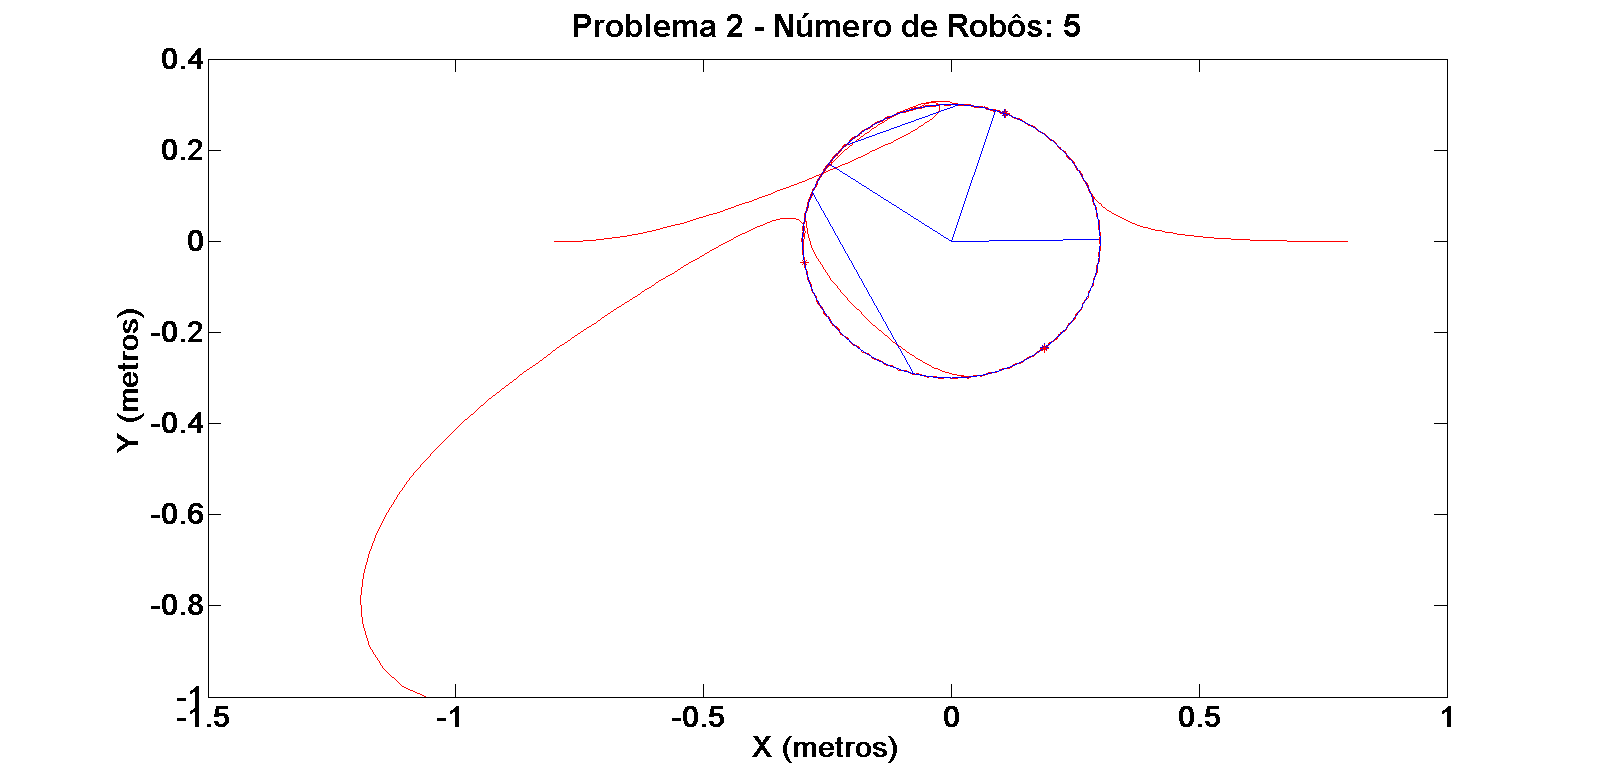
\includegraphics[width=.9\linewidth]{./04-figuras/Simulacoes/Problema2/Falha/P2FalhaFim}
		\caption{Segundo Problema - Falha de 2 Robôs e Reajuste da Formação}
		\label{fig:P2SF2}
	\end{subfigure}
	\caption{Segundo Problema sem Medidas para Evitamento de Colisão}
	\label{fig:sP2F}
\end{figure}

\begin{figure}[!htb]
	\centering
	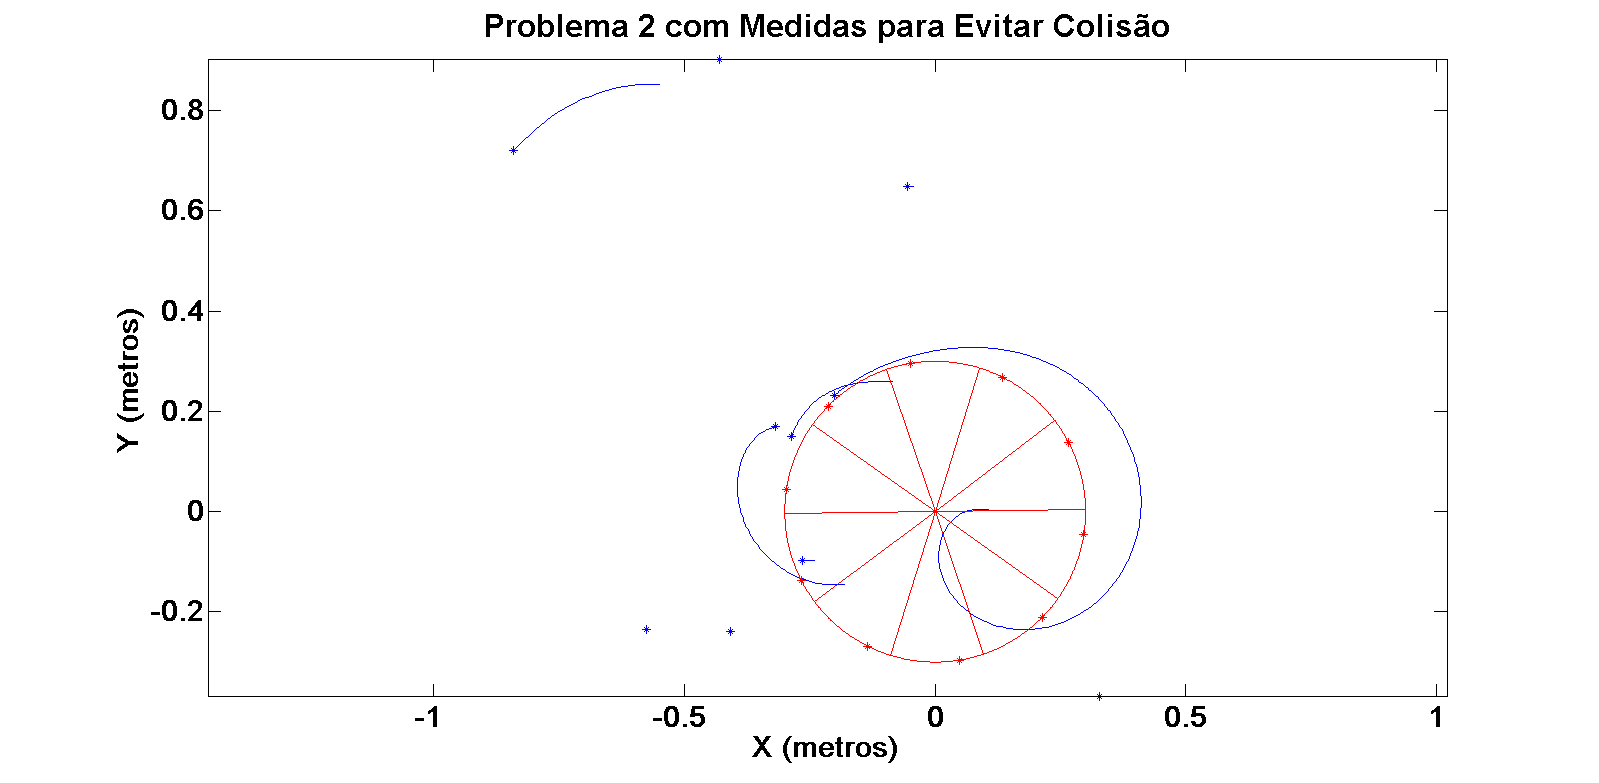
\includegraphics[width=.9\linewidth]{./04-figuras/Simulacoes/Problema2/Colisao/P2_C1}
	\caption{Problema 2: Robôs convergindo um de cada vez, de acordo com a ordem de prioridade}
	\label{fig:P2C}
\end{figure}
            % Simulações
    %%
% Documento: Resultados
%

\chapter{Resultados Esperados}

Espera-se com esse trabalho estudar algumas estratégias de controle de formação de robôs móveis, bem como conhecer as limitações da plataforma \emph{LEGO Mindstorms} para implementação dessas estratégias em um sistema multiagente, explorando-se o comportamento do sistema ao se deparar com falhas em um ou mais robôs.  

%\section{Situação atual}

%Inserir seu texto aqui...

%\section{Análise dos dados coletados}

%Inserir seu texto aqui...
            % Resultados
    \chapter{Conclusão}
\label{chap:conclusao}

Neste trabalho fez-se o estudo de duas estratégias de controle de formação, tendo como intuito a implementação dessas estratégias não só através de simulações como também, com o intuito de desenvolver e aplicar essas estratégias em uma plataforma de baixo custo, o \emph{Lego Mindstorms\textregistered},  

O primeiro problema visava uma espécie de varredura em paralelo por uma frotas de robôs que deveriam se alinhar e seguir se deslocando em conjunto. Já o segundo problema tinha como o objetivo controlar uma tropa de robôs para que a mesma localizasse determinado alvo e a partir daí o circundassem, mantendo uma formação circular e equidistante entre si. Visando uma melhor cobertura da fronteira, a tropa deveria se reajustar caso um ou mais robôs fossem retirados da formação, de modo que a tropa continuasse equidistante porém, circulando o alvo em um período menor, cobrindo melhor a fronteira.

Uma parte deste trabalho foi adaptar as estratégias e soluções encontradas para se adequar a plataforma que apresenta algumas limitações, como por exemplo a da estrutura da rede de comunicação. Uma das limitações deste trabalho, é por exemplo o fato de que a odometria é feita única e exclusivamente, pelos \emph{encoders} já acoplados aos motores da plataforma. Que se mostraram, após todos os testes e experimentos realizados, suficientemente precisos para serem utilizados como ferramenta de medição e alimentação do sistema. 

Entretanto, é necessário cautela quando for realizar mudanças bruscas de velocidade, isso pode ocasionar em derrapagens, fazendo com que o sistema perca sua localização. E como não há nenhum meio externo, uma câmera ou algo para que o robô possa-se localizar novamente, o erro ocorrido vai sendo arrastado até o final da execução do programa, comprometendo o objetivo da frota.

Outra parte importante para o estudo das estratégias de controle de formação foram as simulações realizadas que, apesar de não serem simulações realísticas que levam em consideração muitas características do sistema no mundo real, foram de extrema importância para a abstração das implementações das estratégias. Embora, considerassem o robô como um elemento pontual que ele não é, as simulações foram suficientes para verificar a viabilidade da estratégia adotada e se mostrou uma maneira fácil de verificar o comportamento do sistema para diversas estratégias, contribuindo significamente para a conclusão deste trabalho.

No decorrer deste trabalho foram testados alguns controladores distintos e ajustado empiricamente diversos ganhos para um controlador PID que atendesse aos requisitos do sistema e o que pode-se contatar é que embora alguns controladores demostraram erros menores ou tempo de ajuste inferiores, o que determinou o melhor controlador para o problema foi um custo benefício entre erro, tempo de ajuste e também, suavidade de controle. 

No geral, o controlador da malha interna que melhor atendeu e cumpriu com o objetivo deste trabalho, foi o controlador, aqui denominado como polinomial. % Este controlador consiste em uma função polinomial que converte a velocidade angular desejada em uma variável de potência dos motores, que foi mapeada pelo fabricante em um intervalo de -100 a 100, para que então um controlador PID já ajustado pelo fabricante  
Este controlador é na verdade, um controlador PID já implementado e ajustado pelo fabricante, o ajuste polinomial foi utilizado somente para se obter uma função que traduza o valor de referência (\emph{set point}) aceito pelo controlador do fabricante em velocidade angular das rodas. Já na malha intermediária, um controlador proporcional se mostrou suficiente para cumprir com os objetivos deste trabalho, ao passo que ao inserir um ganho integrador no sistema, o mesmo se mostrou instável.

Foram realizados neste trabalho apenas testes com implementações em uma frota de dois robôs, no entanto, seria interessante como trabalho futuro, aplicar este estudo a uma frota de quatro robôs, como o suportado pela rede de comunicação implementada pela plataforma. 

\section{Trabalhos Futuros}
 \label{sec:trabFuturos}
 Como trabalhos futuros sugere-se a implementação de um tratamento de colisão que, embora não implementado neste trabalho, é parte essencial de um controle de formação. Visto que para cumprir com um objetivo real as tropas devem ser capazes de trabalhar em conjunto sem que um robô atrapalhe na ação de outro e prejudique no desempenho da frota. A inserção de sensores e de uma malha de controle para que o robô consiga interagir com o ambiente, de modo a tornar o controle de formação mais eficiente e mais próximo aos sistemas que resolvem problemas no mundo real.
 
 Outro trabalho interessante seria fazer robôs que se comportem como indivíduos inteligentes e autônomos, capazes de realizar missões sem um grupo mas também, capazes de se organizarem em uma sociedade que possui objetivos em comum e é capaz de decidir pela "melhor" estratégia de formação para cada problema.
 
 
             % Conclusão

    % Elementos pós textuais
    \postextual
    %
% Documento: Referências Bibliográficas
%

\bibliography{./refbase}    % Geração automática das referências por meio do arquivo 'refbase.bib'


       % Referências
    %%
% Documento: Apêndices
%

\begin{apendicesenv}
\partapendices

\chapter{Nome do Apêndice}
\label{chap:apendicex}

Inserir seu texto aqui...

\chapter{Nome do Apêndice}
\label{chap:apendicey}

Inserir seu texto aqui...

\end{apendicesenv}
         % Apêndices
    %%
% Documento: Anexos
%

\begin{anexosenv}
\partanexos

\chapter{Nome do Anexo}
\label{chap:anexox}

Inserir seu texto aqui...

\chapter{Nome do Anexo}
\label{chap:anexoy}

Inserir seu texto aqui...

\end{anexosenv}
            % Anexos
    %\printindex                                             % Índice remissivo

\end{document}
